% \documentclass[handout,xcolor=pdftex,dvipsnames,table]{beamer}
\documentclass{beamer}

\usetheme[framenumber]{AP}

\usepackage[dutch]{babel}
\usepackage{pdfpages}

% Remove the navigation symbols
\beamertemplatenavigationsymbolsempty 

\AtBeginSubsection[]
{
  \begin{frame}<beamer>
    \frametitle{Overzicht}
    \tableofcontents[currentsection,currentsubsection]
  \end{frame}
}

\AtBeginSection[]
{
  \begin{frame}<beamer>
    \frametitle{Overzicht}
    \tableofcontents[currentsection,currentsubsection]
  \end{frame}
}

\title[]{\LaTeX}
\subtitle{A document preparation system}
\author{}
\institute{Jeroen Doggen \\ jeroen.doggen@artesis.be}
\date{Versie: \today}

\begin{document}

% Titlepage 
\maketitle

% Outline Page
\section*{Overzicht}
\begin{frame}
\frametitle{Overzicht}
\tableofcontents
\end{frame}

%%%%%%%%%%%%%%%%%%%%%%%%%%%%%%%%%%%%%%%%%%%%%%%%%%%%%%%%%%%%%%%%%%%%%%%%%%%%%%%%%%%%%%%%%%%%%%%%%%%%%%%%%%%%%%%%%%%%%%%%%%%%%%%%%%%%
\section{\LaTeX}
%%%%%%%%%%%%%%%%%%%%%%%%%%%%%%%%%%%%%%%%%%%%%%%%%%%%%%%%%%%%%%%%%%%%%%%%%%%%%%%%%%%%%%%%%%%%%%%%%%%%%%%%%%%%%%%%%%%%%%%%%%%%%%%%%%%%
\subsection{Achtergrond}
%%%%%%%%%%%%%%%%%%%%%%%%%%%%%%%%%%%%%%%%%%%%%%%%%%%%%%%%%%%%%%%%%%%%%%%%%%%%%%%%%%%%%%%%%%%%%%%%%%%%%%%%%%%%%%%%%%%%%%%%%%%%%%%%%%%%

\begin{frame}
\frametitle{Wat is \LaTeX?}
\begin{itemize}[<+->]
 \item \LaTeX is een ``typesetting'' systeem, voor teksten, documenten en wiskundige formule
 \item ``TEX'', de basisbouwsteen van het \LaTeX systeem werd geschreven door Donald Ervin Knuth \footnote{Bekende computerwetenschapper, auteur van ``The Art of Computer Programming'', \url{http://www-cs-faculty.stanford.edu/~knuth}}
 \item  De ``X'' is \LaTeX staat voor de Griekse letter $\chi$ (Chi) en wordt dus als ``Tech'' uitgesproken
 \begin{itemize}
  \item Niet zoals de handschoenen / vrijetijdskleding
  \end{itemize}

\end{itemize}
\begin{figure}[h] 
  
\includegraphics[width=0.5\textwidth]{images/latex.png}
\end{figure}
\end{frame}

%%%%%%%%%%%%%%%%%%%%%%%%%%%%%%%%%%%%%%%%%%%%%%%%%%%%%%%%%%%%%%%%%%%%%%%%%%%%%%%%%%%%%%%%%%%%%%%%%%%%%%%%%%%%%%%%%%%%%%%%%%%%%%%%%%%%

\begin{frame}
\frametitle{Wat is typesetting?}
\begin{columns}[c] 
\column{.4\textwidth} 
\begin{figure}[h] 
  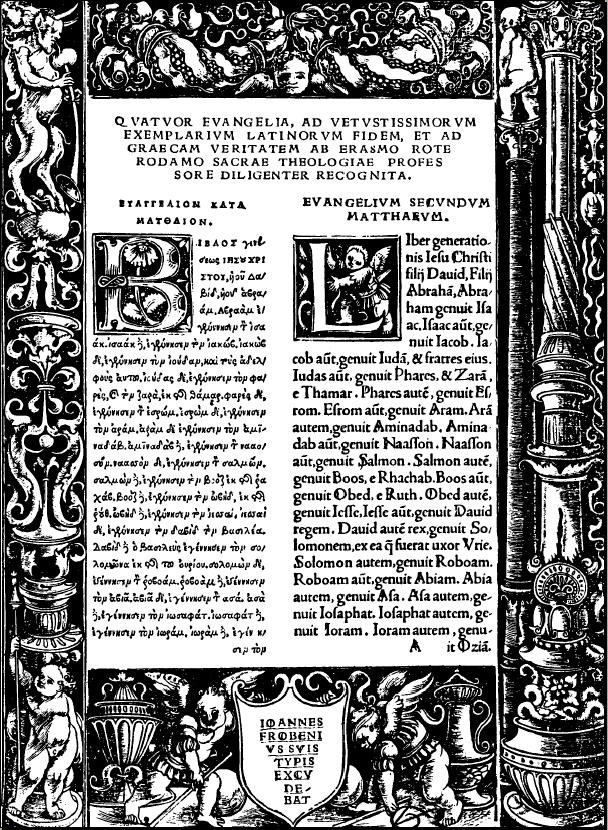
\includegraphics[width=1\textwidth]{images/typesetting.png}
\end{figure}
\column{.65\textwidth}
\begin{itemize}
 \item <1-> Het maken van (mooie/goede) documenten.
 \begin{itemize}
  \item Mooie lettertypen
  \item Duidelijke structuur
  \item Conform standaarden en afspraken
 \end{itemize}
 \item <2-> Was vroeger een zeer complex proces.
 \item <3-> Een goed document maken is nog steeds een kunst.
 \item <4-> Maar omdat de meesten onder ons geen kunstenaars zijn...
 \item <4-> ... gebruiken we hiervoor software.
 \item <4-> ... \LaTeX
\end{itemize}
\end{columns}
\end{frame}

%%%%%%%%%%%%%%%%%%%%%%%%%%%%%%%%%%%%%%%%%%%%%%%%%%%%%%%%%%%%%%%%%%%%%%%%%%%%%%%%%%%%%%%%%%%%%%%%%%%%%%%%%%%%%%%%%%%%%%%%%%%%%%%%%%%%

\begin{frame}
\frametitle{Traditionele workflow voor publiceren}
\begin{enumerate}
 \item <1-> De \textbf{auteur} geeft een manuscript aan een uitgeverij
 \item <2-> De \textbf{boek designer} van de uitgeverij beslist over de layout van het document (kolombreedte, fonts, ...)
 \item <3-> De boek designer schrijf zijn instructies neer in een document en geeft deze aan een typesetter.
 \item <4-> De \textbf{typesetter} ontwerpt het boek op basis van deze instructies.
\end{enumerate}

\begin{itemize}[<+->]
 \item <5-> De \textbf{boek designer} probeert op basis van zijn ervaring en door overleg met de auteur een optimaal resultaat te bekomen.
 \item <5-> Zijn beslissingen i.v.m. hoofdstukken, citaties, formules ... hangen af van: professionele ervaring, type van het manuscript, doelpubliek, plek van publicatie,... 
\end{itemize}
\end{frame}

%%%%%%%%%%%%%%%%%%%%%%%%%%%%%%%%%%%%%%%%%%%%%%%%%%%%%%%%%%%%%%%%%%%%%%%%%%%%%%%%%%%%%%%%%%%%%%%%%%%%%%%%%%%%%%%%%%%%%%%%%%%%%%%%%%%%

\begin{frame}[fragile] 
\frametitle{Geautomatiseerde workflow}
\LaTeX neemt de rol van boek designer over en gebruikt TeX als de typsetter
\begin{itemize}[<+->]
 \item \LaTeX is slechts software en heeft dus iets meer instructies nodig.
 \item De auteur moet extra informatie aan zijn tekst toevoegen om de \textbf{logische structuur} van zijn werk te beschrijven.
 \item De informatie wordt in het ASCII manuscript opgenomen als \LaTeX commando's
 \item Deze zijn vergelijkbaar met HTML commando's
 \begin{itemize}
 \item jammer genoeg zijn ook enkele problemen van HTML hier een mogelijk probleem
  \begin{verbatim}
  je zou kunnen schrijven:
    <FONT SIZE=“+3” FACE=“ARIAL”><B>Heading</B></FONT>
  of toch beter: 
    <H1>Heading</H1>
 \end{verbatim}
\end{itemize}
\end{itemize}
\end{frame}

%%%%%%%%%%%%%%%%%%%%%%%%%%%%%%%%%%%%%%%%%%%%%%%%%%%%%%%%%%%%%%%%%%%%%%%%%%%%%%%%%%%%%%%%%%%%%%%%%%%%%%%%%%%%%%%%%%%%%%%%%%%%%%%%%%%%

\begin{frame}
\frametitle{Standaard \LaTeX workflow}
\begin{itemize}
 \item Schrijf een inputfile: 
    \begin{enumerate}
      \item Opmaak van het document: normaal via een standaard sjabloon dat je zelden zal moeten aanpassen
      \item Definieer de structuur van het document
      \item Schijf de inhoud van het document
      \item Wordt omgezet in het uiteindelijke document door \LaTeX.
      \end{enumerate}
\pause
 \item Traditionele ``WYSIWYG\footnote{acroniem voor What You See Is What You Get} tekstverwerker'' stap 1,2,3 worden constant uitgevoerd (in theorie niet, in de praktijk wel...) 
    \begin{itemize}
    \item Dit is tijdsverlies(?), irritant(?), niet logisch(?),...
      \end{itemize}
\end{itemize}
\begin{figure}[h] 
  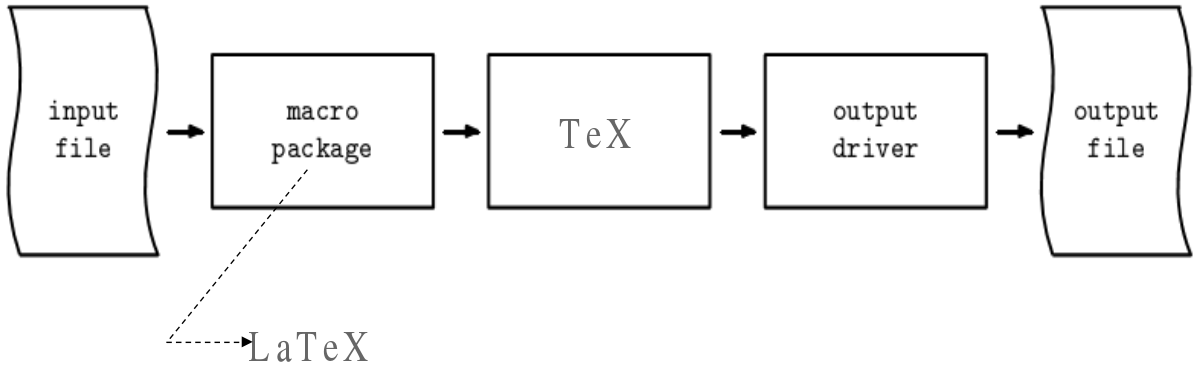
\includegraphics[width=0.8\textwidth]{images/workflow.png}
\end{figure}
\end{frame}

%%%%%%%%%%%%%%%%%%%%%%%%%%%%%%%%%%%%%%%%%%%%%%%%%%%%%%%%%%%%%%%%%%%%%%%%%%%%%%%%%%%%%%%%%%%%%%%%%%%%%%%%%%%%%%%%%%%%%%%%%%%%%%%%%%%%

\begin{frame}
\frametitle{Layout design}
Typografisch design is een kunst
\begin{itemize}[<+->]
 \item <1-> Auteurs zonder ervaring maken vaak serieuze opmaakfouten door aan te nemen dat boek ontwerp enkel over esthetische aspecten gaat.
    \begin{itemize}
    \item Als een document en mooi uitziet zal het ook wel een goed document zijn.... \textit{dit is niet waar!}
    \end{itemize}
 \item <2-> Een document moet gelezen worden, niet in een kader aan de muur worden gehangen.
 \item <3-> De leesbaarheid en begrijpbaarheid van een document zijn belangrijker dan het uiterlijk:
    \begin{itemize}
    \item Fonts en nummering van hoofdstukken moet zo gekozen worden dat ze de structuur van hoofdstukken meteen op een visuele manier duidelijk maken aan de lezer.
    \item De lengte van een regel moet lang genoeg zijn, maar ook niet te kort. (visuele aspect vs nuttige aspect)
    \end{itemize}
\end{itemize}
\end{frame}

%%%%%%%%%%%%%%%%%%%%%%%%%%%%%%%%%%%%%%%%%%%%%%%%%%%%%%%%%%%%%%%%%%%%%%%%%%%%%%%%%%%%%%%%%%%%%%%%%%%%%%%%%%%%%%%%%%%%%%%%%%%%%%%%%%%%

\begin{frame}
\frametitle{Voorbeeld}
Is het overzicht hier nog steeds duidelijk?

\begin{figure}[h] 
  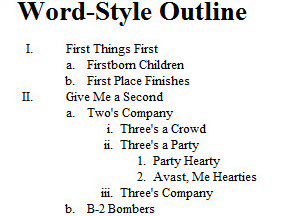
\includegraphics[width=0.5\textwidth]{images/indent.jpg}
\end{figure}
\end{frame}

%%%%%%%%%%%%%%%%%%%%%%%%%%%%%%%%%%%%%%%%%%%%%%%%%%%%%%%%%%%%%%%%%%%%%%%%%%%%%%%%%%%%%%%%%%%%%%%%%%%%%%%%%%%%%%%%%%%%%%%%%%%%%%%%%%%%

\begin{frame}
\frametitle{Layout design}
\begin{itemize}
 \item <1->Met WYSIWYG systemen worden vaak h\'e\'el mooie documenten, met h\'e\'el weinig of een inconsistente structuur gemaakt.
 \item <2->\LaTeX verhindert deze ``formatting errors'' door de auteur te forceren om de logisch structuur van het document vast te leggen. (en dus moet je er ook over nadenken...)
 \begin{itemize}
  \item Op basis van de logische structuur zal de layout automatisch worden aangepast.
 \end{itemize}
 \item <3->Logische mark-up verhoogt de draagbaarheid van documenten.
 \begin{itemize}
  \item Tijdschriften en uitgevers kunnen stylesheets gebruiken om de logische markup om te zetten in (visueel) verschillende documenten met dezelfde inhoud rekening houdend met hun in-house stylesheet.
 \end{itemize}
 \end{itemize}
\end{frame}

%%%%%%%%%%%%%%%%%%%%%%%%%%%%%%%%%%%%%%%%%%%%%%%%%%%%%%%%%%%%%%%%%%%%%%%%%%%%%%%%%%%%%%%%%%%%%%%%%%%%%%%%%%%%%%%%%%%%%%%%%%%%%%%%%%%%

\begin{frame}
\frametitle{Voorbeeld stylesheet}
\begin{figure}[hb] 
  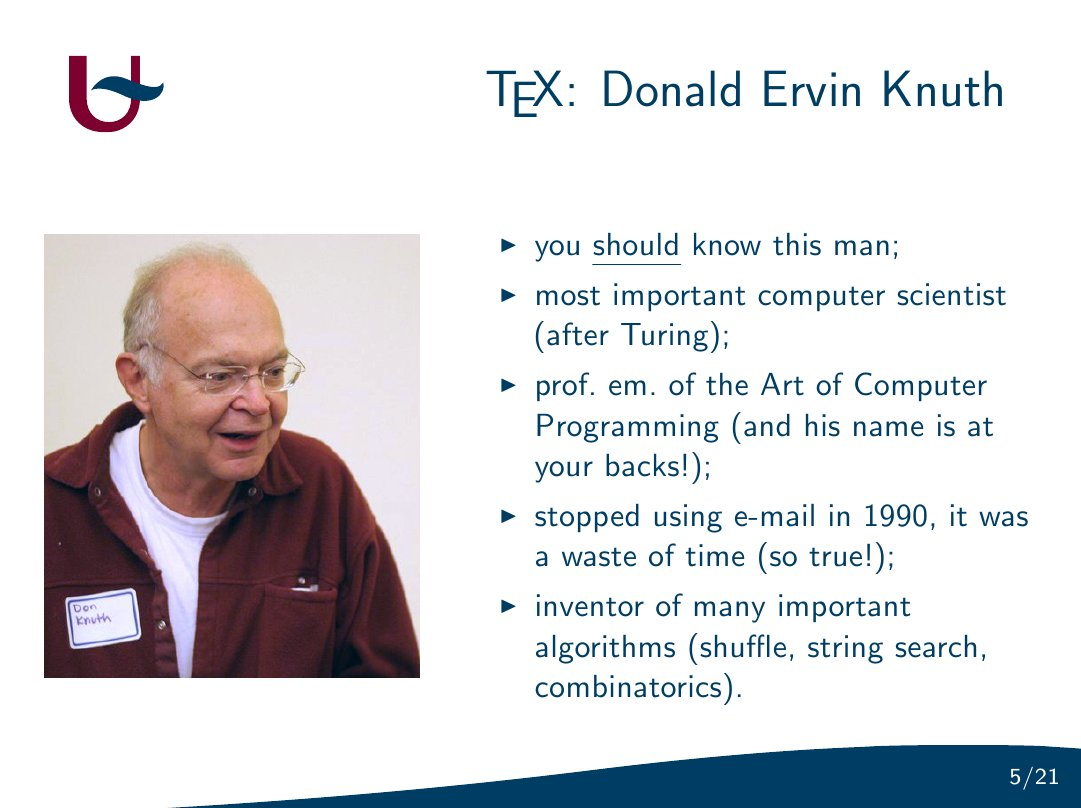
\includegraphics[width=0.85\textwidth]{images/knuth.jpeg}
\end{figure}
\end{frame}

%%%%%%%%%%%%%%%%%%%%%%%%%%%%%%%%%%%%%%%%%%%%%%%%%%%%%%%%%%%%%%%%%%%%%%%%%%%%%%%%%%%%%%%%%%%%%%%%%%%%%%%%%%%%%%%%%%%%%%%%%%%%%%%%%%%%

\begin{frame}
\frametitle{Voordelen van \LaTeX}
\begin{itemize}
 \item Professionele opmaakprofielen zijn beschikbaar
 \item Standaard voor wetenschappelijke documenten
 \item Verwerken van wiskundige en andere speciale symbolen
 \item Betekenis gebaseerde structurering (i.p.v. uiterlijk gebaseerde)
 \item Gigantische online user community
\end{itemize}
\begin{figure}[hb] 
  
\includegraphics[width=0.5\textwidth]{images/lion.png}
\end{figure}

\end{frame}

%%%%%%%%%%%%%%%%%%%%%%%%%%%%%%%%%%%%%%%%%%%%%%%%%%%%%%%%%%%%%%%%%%%%%%%%%%%%%%%%%%%%%%%%%%%%%%%%%%%%%%%%%%%%%%%%%%%%%%%%%%%%%%%%%%%%

\begin{frame}
\frametitle{Voordelen van \LaTeX}
\begin{itemize}
 \item Gebruikers moeten enkel een set basiscommando's kennen om te starten, enkel voor geavanceerde opties is meer kennis nodig
 \item Complexe structuren zoals voetnoten, referenties, inhoudstafels en bibliografieen kunnen automatisch aangemaakt worden
 \item Voor veel typografische zaken die niet met standaard \LaTeX mogelijk zijn bestaan er extensies.
 \item Spoort auteurs aan om goed gestructureerde documenten te schrijven.
 \item Gratis en platform onafhankelijk
\end{itemize}
\begin{figure}[h] 
  
\includegraphics[width=0.15\textwidth]{images/bsd.png}
  
\includegraphics[width=0.5\textwidth]{images/indep.jpg}
\end{figure}
\end{frame}

%%%%%%%%%%%%%%%%%%%%%%%%%%%%%%%%%%%%%%%%%%%%%%%%%%%%%%%%%%%%%%%%%%%%%%%%%%%%%%%%%%%%%%%%%%%%%%%%%%%%%%%%%%%%%%%%%%%%%%%%%%%%%%%%%%%%

\begin{frame}
\frametitle{Nadelen van \LaTeX}
\begin{itemize}
 \item Slecht gestructureerde documenten schrijven is moeilijk.
 \item De leercurve is in het begin frustrerend.
 \item Aanpassen om net te krijgen wat je wil hebben is lastig.
 \begin{itemize}
  \item Is wat je wil wel een goed plan vanuit ``layout'' standpunt?
 \end{itemize}
 \item Het aanmaken van sjablonen en stylesheets is lastig.
 \item ``What you see is \textbf{not} what you get''
 \begin{itemize}
  \item Is dit een nadeel? Waarom ben je aan het nadenken over layout tijdens het schrijven... i.p.v. na te denken over de inhoud?
 \end{itemize}
\end{itemize}
\begin{figure}[h] 
  
\includegraphics[width=0.42\textwidth]{images/dummy.jpg}
\end{figure}
\end{frame}

%%%%%%%%%%%%%%%%%%%%%%%%%%%%%%%%%%%%%%%%%%%%%%%%%%%%%%%%%%%%%%%%%%%%%%%%%%%%%%%%%%%%%%%%%%%%%%%%%%%%%%%%%%%%%%%%%%%%%%%%%%%%%%%%%%%%
\subsection{Praktisch}
%%%%%%%%%%%%%%%%%%%%%%%%%%%%%%%%%%%%%%%%%%%%%%%%%%%%%%%%%%%%%%%%%%%%%%%%%%%%%%%%%%%%%%%%%%%%%%%%%%%%%%%%%%%%%%%%%%%%%%%%%%%%%%%%%%%%

\begin{frame}
\frametitle{Bron bestanden}
\begin{itemize}
 \item Je vertrek van zuivere ASCII bestanden.
 \item Kan geschreven worden met iedere tekst editor.
 \pause
 \item Dit bestand bevat:
 \begin{itemize}
  \item De tekst van het document: inhoud
  \item Commando's die aan \LaTeX vertellen hoe het typesetting proces moet verlopen
  \begin{itemize}
   \item Titels, hoofdstukken, bibliografieen
   \item Formules, speciale karakters, afbeeldingen, tabellen
   \item Complexere commando's, commentaar, witruimten,...   
  \end{itemize}
 \end{itemize}
\end{itemize}
\end{frame}

%%%%%%%%%%%%%%%%%%%%%%%%%%%%%%%%%%%%%%%%%%%%%%%%%%%%%%%%%%%%%%%%%%%%%%%%%%%%%%%%%%%%%%%%%%%%%%%%%%%%%%%%%%%%%%%%%%%%%%%%%%%%%%%%%%%%

\begin{frame}
\frametitle{Witruimte}
\begin{itemize}
 \item <1-> Alle ``witruimte'' karakters worden door \LaTeX hetzelfde behandeld: ze worden omgezet in \'e\'en spatie.
    \begin{itemize}
      \item Meerdere spaties en tabs worden omgezet in \'e\'en spatie.
    \end{itemize}
 \item <2-> Een lege lijn tussen twee lijnen tekst wordt gezien als het einde van een paragraaf. (begin de volgende zin op een nieuwe regel)
      \begin{itemize}
      \item Meerdere lege lijnen worden behandeld alsof er \'e\'en lege lijn staat.
      \end{itemize}
\end{itemize}
\begin{figure}[h] 
  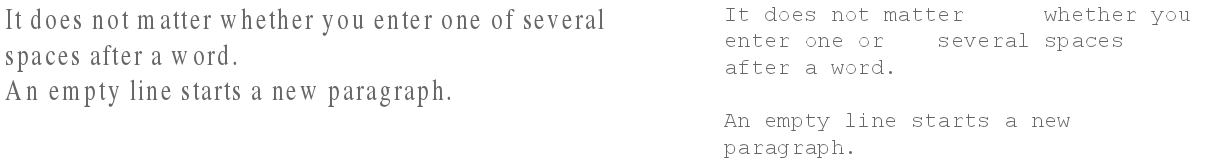
\includegraphics[width=1\textwidth]{images/spaces.png}
\end{figure}
\end{frame}

%%%%%%%%%%%%%%%%%%%%%%%%%%%%%%%%%%%%%%%%%%%%%%%%%%%%%%%%%%%%%%%%%%%%%%%%%%%%%%%%%%%%%%%%%%%%%%%%%%%%%%%%%%%%%%%%%%%%%%%%%%%%%%%%%%%%

\begin{frame}
\frametitle{Speciale karakters}
\begin{itemize}
 \item Enkele karakters hebben een speciale functie: \$, \&, \%, \#, \{, \}
 \item Enkele van deze symbolen kunnen in uw tekst ingevoegd worden door een ``\textbackslash'' voor het symbool te plaatsen.
 \item Deze en vele andere symbolen kunnen met speciale commando's geplaatst worden.
\end{itemize}
\end{frame}

%%%%%%%%%%%%%%%%%%%%%%%%%%%%%%%%%%%%%%%%%%%%%%%%%%%%%%%%%%%%%%%%%%%%%%%%%%%%%%%%%%%%%%%%%%%%%%%%%%%%%%%%%%%%%%%%%%%%%%%%%%%%%%%%%%%%

\begin{frame}
\frametitle{Opmaak commando's}
\begin{itemize}
 \item De commando's zijn case-sensitive en bestaan in twee formaten:
      \begin{itemize}
      \item Ze starten met een backslash ``\textbackslash'' en bestaan uit enkele letters
      \item Sommige commando's aanvaarden parameters tussen accolades en eventueel extra/optionele parameters tussen vierkante haken.
     \end{itemize}
\end{itemize}
\begin{figure}[h] 
  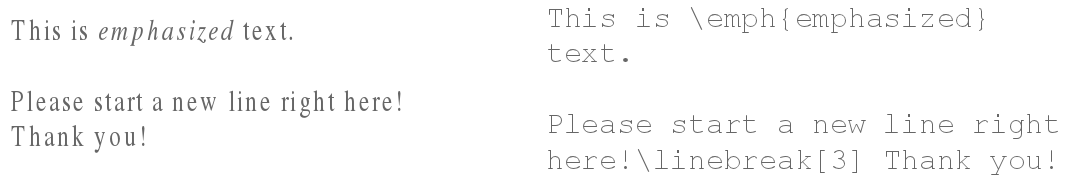
\includegraphics[width=1\textwidth]{images/command.png}
\end{figure}
\end{frame}

%%%%%%%%%%%%%%%%%%%%%%%%%%%%%%%%%%%%%%%%%%%%%%%%%%%%%%%%%%%%%%%%%%%%%%%%%%%%%%%%%%%%%%%%%%%%%%%%%%%%%%%%%%%%%%%%%%%%%%%%%%%%%%%%%%%%

\begin{frame}
\frametitle{Commentaar}
\begin{itemize}
 \item Wanneer \% karakter op een regel staat, dan wordt de rest van de regel automatisch als commentaar gezien.
 \item Dit is handig om notities rechtstreeks in de tekst toe te voegen, zonder dat deze in het finale bestand terechtkomen.
\end{itemize}
\begin{figure}[h] 
  
\includegraphics[width=1\textwidth]{images/comment.png}
\end{figure}
\end{frame}

%%%%%%%%%%%%%%%%%%%%%%%%%%%%%%%%%%%%%%%%%%%%%%%%%%%%%%%%%%%%%%%%%%%%%%%%%%%%%%%%%%%%%%%%%%%%%%%%%%%%%%%%%%%%%%%%%%%%%%%%%%%%%%%%%%%%

\begin{frame}
\frametitle{Opbouw bronbestand}
\begin{itemize}[<+->]
 \item Een elementair bestand heeft volgende opbouw:
 \begin{figure}[h] 
  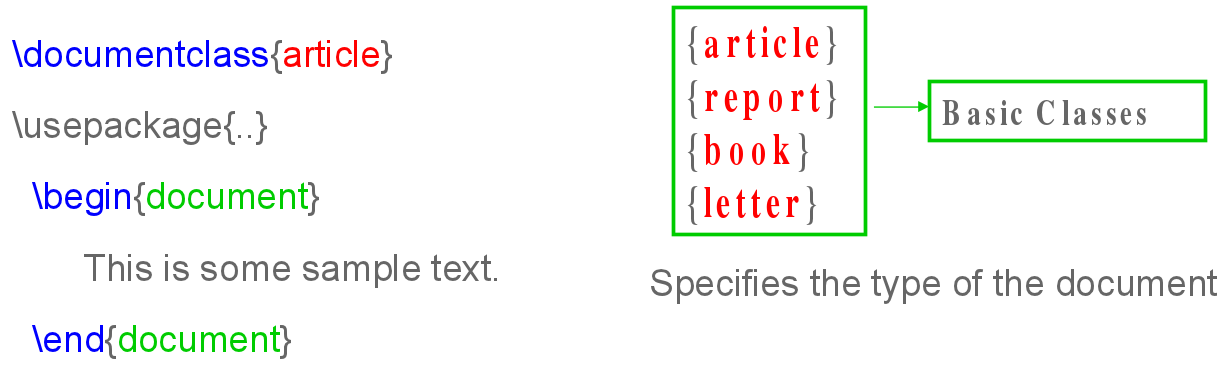
\includegraphics[width=0.9\textwidth]{images/bestand.png}
\end{figure}
 \item Aanmaken documentstructuur / hoofdstukken:
  \begin{figure}[h] 
  
\includegraphics[width=0.5\textwidth]{images/sections.png}
\end{figure}
\end{itemize}
\end{frame}

%%%%%%%%%%%%%%%%%%%%%%%%%%%%%%%%%%%%%%%%%%%%%%%%%%%%%%%%%%%%%%%%%%%%%%%%%%%%%%%%%%%%%%%%%%%%%%%%%%%%%%%%%%%%%%%%%%%%%%%%%%%%%%%%%%%%

\begin{frame}
\frametitle{Opbouw bronbestand}
\begin{itemize}[<+->]
 \item Invoegen van een afbeelding uit een bestand:
 \begin{figure}[h] 
  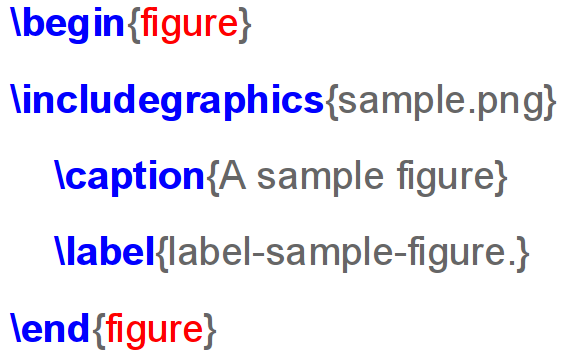
\includegraphics[width=0.37\textwidth]{images/figure.png}
\end{figure}
 \item Invoegen van een tabel: (vector)
  \begin{figure}[h] 
  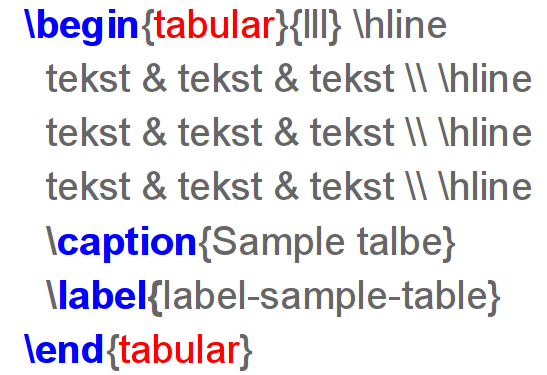
\includegraphics[width=0.4\textwidth]{images/tabel.png}
\end{figure}
\end{itemize}
\end{frame}

%%%%%%%%%%%%%%%%%%%%%%%%%%%%%%%%%%%%%%%%%%%%%%%%%%%%%%%%%%%%%%%%%%%%%%%%%%%%%%%%%%%%%%%%%%%%%%%%%%%%%%%%%%%%%%%%%%%%%%%%%%%%%%%%%%%%

\begin{frame}
\frametitle{Cross referenties}
\begin{itemize}[<+->]
 \item Om binnen je tekst te verwijzen naar andere ``objecten'' binnen je tekst. (afbeeldingen, hoofdstukken, formules, tabellen,...)
\end{itemize}
  \begin{figure}[h] 
    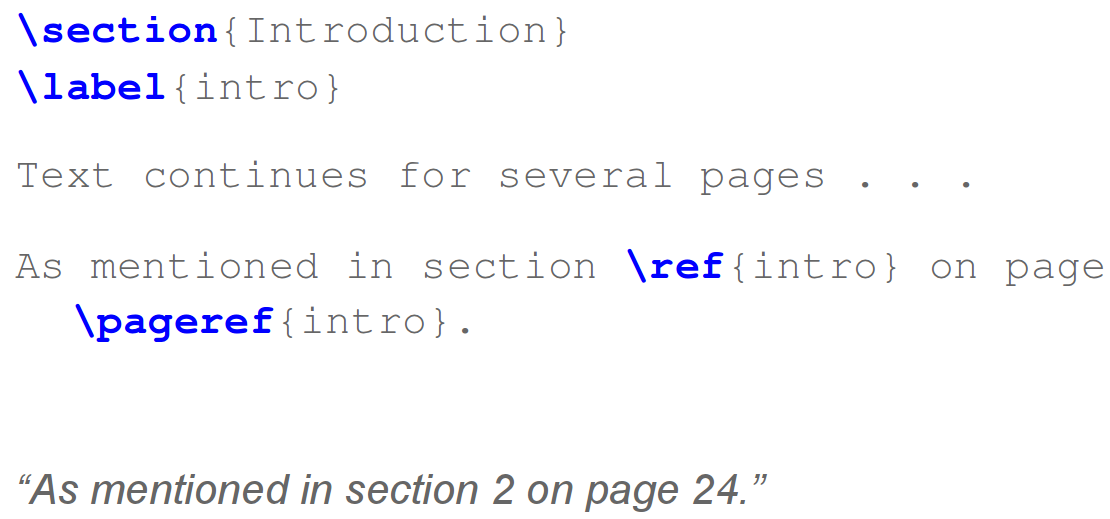
\includegraphics[width=0.8\textwidth]{images/reference.png}
  \end{figure}
\end{frame}

%%%%%%%%%%%%%%%%%%%%%%%%%%%%%%%%%%%%%%%%%%%%%%%%%%%%%%%%%%%%%%%%%%%%%%%%%%%%%%%%%%%%%%%%%%%%%%%%%%%%%%%%%%%%%%%%%%%%%%%%%%%%%%%%%%%%

\begin{frame}[fragile]
\frametitle{Wiskundige formules}
\begin{itemize}
 \item De zeer goede ondersteuning voor wiskundige formules is \'e\'en van de sterkste punten van \LaTeX.
 \item Iedere denkbare wiskundige formule kan worden opgebouwd, eventueel door extra packages te gebruiken.
 \item Binnen een tekst kan een formule worden ingevoegd door een stuk tekst tussen dollartekens te plaatsen. ``\$ formule \$''
\begin{columns}[c] 
\column{.4\textwidth}
To find the square of the hypotenuse, add a squared to b squared to find c squared, e.g. $a^2 + b^2 = c^2$. It’s as easy as that!
\column{.4\textwidth}
\begin{verbatim}
 To find the square of the 
 hypotenuse, add a squared 
 to b squared to find c 
 squared, e.g. $a^2 + b^2 
 = c^2$. It’s as easy as 
 that!
\end{verbatim}
\end{columns}
\end{itemize}
\end{frame}

%%%%%%%%%%%%%%%%%%%%%%%%%%%%%%%%%%%%%%%%%%%%%%%%%%%%%%%%%%%%%%%%%%%%%%%%%%%%%%%%%%%%%%%%%%%%%%%%%%%%%%%%%%%%%%%%%%%%%%%%%%%%%%%%%%%%

\begin{frame}
\frametitle{Wiskundige formules}
\begin{itemize}
 \item Wikipedia formules worden op de website ook geschreven m.b.v. \LaTeX.
 \item Je kan de formule zien door het ``alternate text'' veld van de afbeelding/formule te bekijken.
 \item ``log normale distributie'': $f_X(x;\mu,\sigma) = \frac{1}{x \sigma \sqrt{2 \pi}}\, e^{-\frac{(\ln x - \mu)^2}{2\sigma^2}}$
  \begin{figure}[h] 
    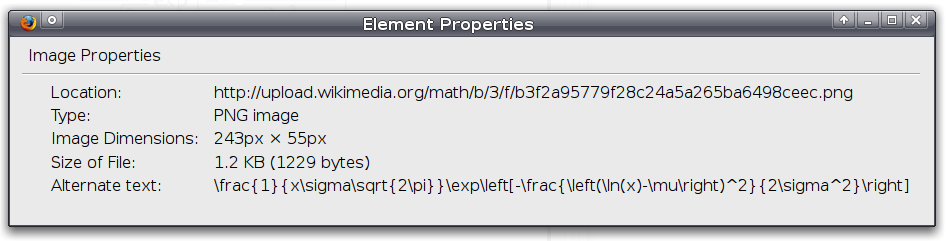
\includegraphics[width=1\textwidth]{images/formulewiki.png}
  \end{figure}
 \end{itemize}
\end{frame}

%%%%%%%%%%%%%%%%%%%%%%%%%%%%%%%%%%%%%%%%%%%%%%%%%%%%%%%%%%%%%%%%%%%%%%%%%%%%%%%%%%%%%%%%%%%%%%%%%%%%%%%%%%%%%%%%%%%%%%%%%%%%%%%%%%%%

\begin{frame}
\frametitle{Bibliografie}
\begin{itemize}
 \item Je kan binnen uw tekst verwijzen naar andere artikels of boeken. Deze zullen dan automatisch worden opgenomen in de bibliografie.
 \item De informatie van de geciteerd artikels worden opgeslagen in een ``.bib'' bestand.
 \item BibTeX is het programma dat wordt aangeroepen om het aanmaken van de bibliografie uit te voeren. (er worden enkele tijdelijke hulpbestanden aangemaakt)
  \begin{figure}[h] 
    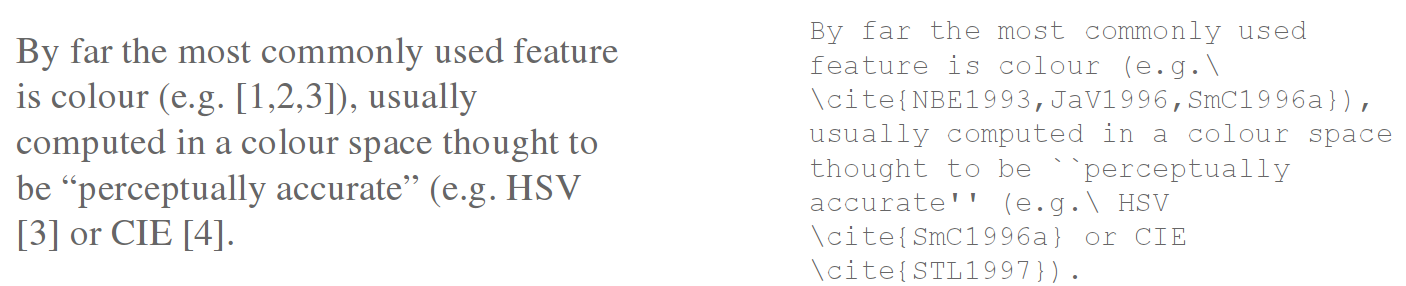
\includegraphics[width=1\textwidth]{images/biblio.png}
  \end{figure}
 \end{itemize}
\end{frame}

%%%%%%%%%%%%%%%%%%%%%%%%%%%%%%%%%%%%%%%%%%%%%%%%%%%%%%%%%%%%%%%%%%%%%%%%%%%%%%%%%%%%%%%%%%%%%%%%%%%%%%%%%%%%%%%%%%%%%%%%%%%%%%%%%%%%

\begin{frame}
\frametitle{Bibliografie}
\begin{itemize}
 \item Voorbeeld van een .bib bestand.
  \begin{figure}[h] 
    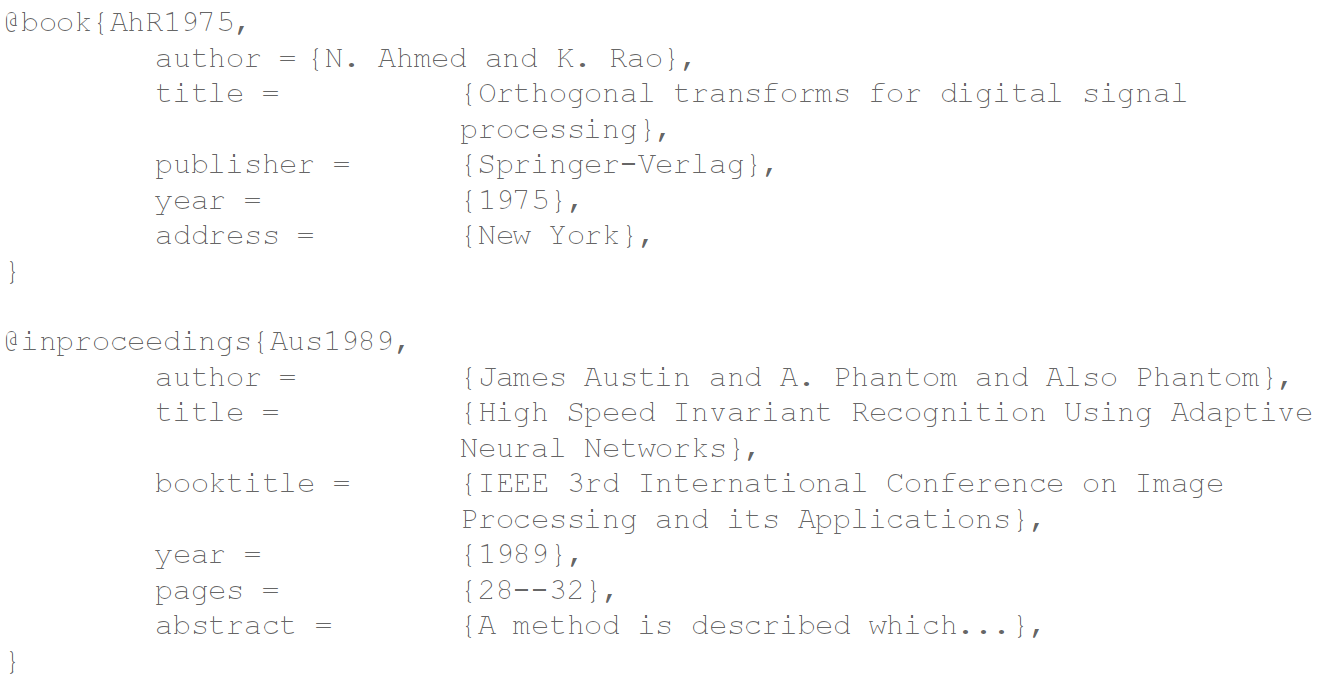
\includegraphics[width=1\textwidth]{images/bibliofile.png}
  \end{figure}
 \end{itemize}
\end{frame}

%%%%%%%%%%%%%%%%%%%%%%%%%%%%%%%%%%%%%%%%%%%%%%%%%%%%%%%%%%%%%%%%%%%%%%%%%%%%%%%%%%%%%%%%%%%%%%%%%%%%%%%%%%%%%%%%%%%%%%%%%%%%%%%%%%%%

\begin{frame}
\frametitle{Output formaten}
\begin{itemize}
 \item Het finale bestand dat wordt gegenereerd kan een aantal formaten hebben: (geen exhaustieve lijst)
\begin{itemize}
 \item .dvi : ``device independent'' formaat: originele formaat van de TeX engine. Werkt zeer snel en handig onder Linux, maar slecht ondersteund onder Windows.
 \item .ps :  vectorieel formaat
 \item .pdf : vectorieel formaat, initieel exclusief van Adobe, nu toch een defacto standaard geworden. (heeft jammer genoeg wel zijn beperkingen)
 \item .html : webpagina, momenteel wordt gewerkt aan een converter om dit om te zetten in .ipub bestanden voor e-book readers
\end{itemize}
 \end{itemize}
\end{frame}

%%%%%%%%%%%%%%%%%%%%%%%%%%%%%%%%%%%%%%%%%%%%%%%%%%%%%%%%%%%%%%%%%%%%%%%%%%%%%%%%%%%%%%%%%%%%%%%%%%%%%%%%%%%%%%%%%%%%%%%%%%%%%%%%%%%%

\begin{frame}
\frametitle{Software tools}
\begin{itemize}
 \item Iedere intellingente ASCII teksteditor / IDE: \textit{ieder zijn eigen voorkeur}
    \begin{itemize}
    \item Windows: TeXnicCenter, ProTeXt, WinEdt (Kile)
    \item Linux: Kile, TeXLive, Geany, Gedit,...
    \item Mac: LyX, MacTex,...
    \end{itemize}
 \item \LaTeX $ $ build engines: Miktex, texlive
\end{itemize}
\end{frame}

%%%%%%%%%%%%%%%%%%%%%%%%%%%%%%%%%%%%%%%%%%%%%%%%%%%%%%%%%%%%%%%%%%%%%%%%%%%%%%%%%%%%%%%%%%%%%%%%%%%%%%%%%%%%%%%%%%%%%%%%%%%%%%%%%%%%

\begin{frame}
\frametitle{Niet besproken}
\begin{itemize}[<+->]
 \item Enkele zaken werden niet besproken in deze inleiding:
    \begin{itemize}
    \item Insluiten van andere .pdf bestanden
    \item Figuren en wiskundige functies tekenen
    \item Slides opstellen \textit{(zoals deze slides)}
    \item Scripting: aanroepen van \LaTeX $ $ van op commandline om complexere bewerkingen mogelijk te maken. \textit{(zoals aanmaken van handout versies van slides, archiveren in .zip bestand,...)}
    \item Zaken die ik vergeten ben of waarvan ik zelf (nog) niet van op de hoogte ben...
    \end{itemize}
\end{itemize}
\end{frame}

%%%%%%%%%%%%%%%%%%%%%%%%%%%%%%%%%%%%%%%%%%%%%%%%%%%%%%%%%%%%%%%%%%%%%%%%%%%%%%%%%%%%%%%%%%%%%%%%%%%%%%%%%%%%%%%%%%%%%%%%%%%%%%%%%%%%




%%%%%%%%%%%%%%%%%%%%%%%%%%%%%%%%%%%%%%%%%%%%%%%%%%%%%%%%%%%%%%%%%%%%%%%%%%%%%%%%%%%%%%%%%%%%%%%%%%%%%%%%%%%%%%%%%%%%%%%%%%%%%%%%%%%%
\subsection{Voorbeeld documenten}
%%%%%%%%%%%%%%%%%%%%%%%%%%%%%%%%%%%%%%%%%%%%%%%%%%%%%%%%%%%%%%%%%%%%%%%%%%%%%%%%%%%%%%%%%%%%%%%%%%%%%%%%%%%%%%%%%%%%%%%%%%%%%%%%%%%%
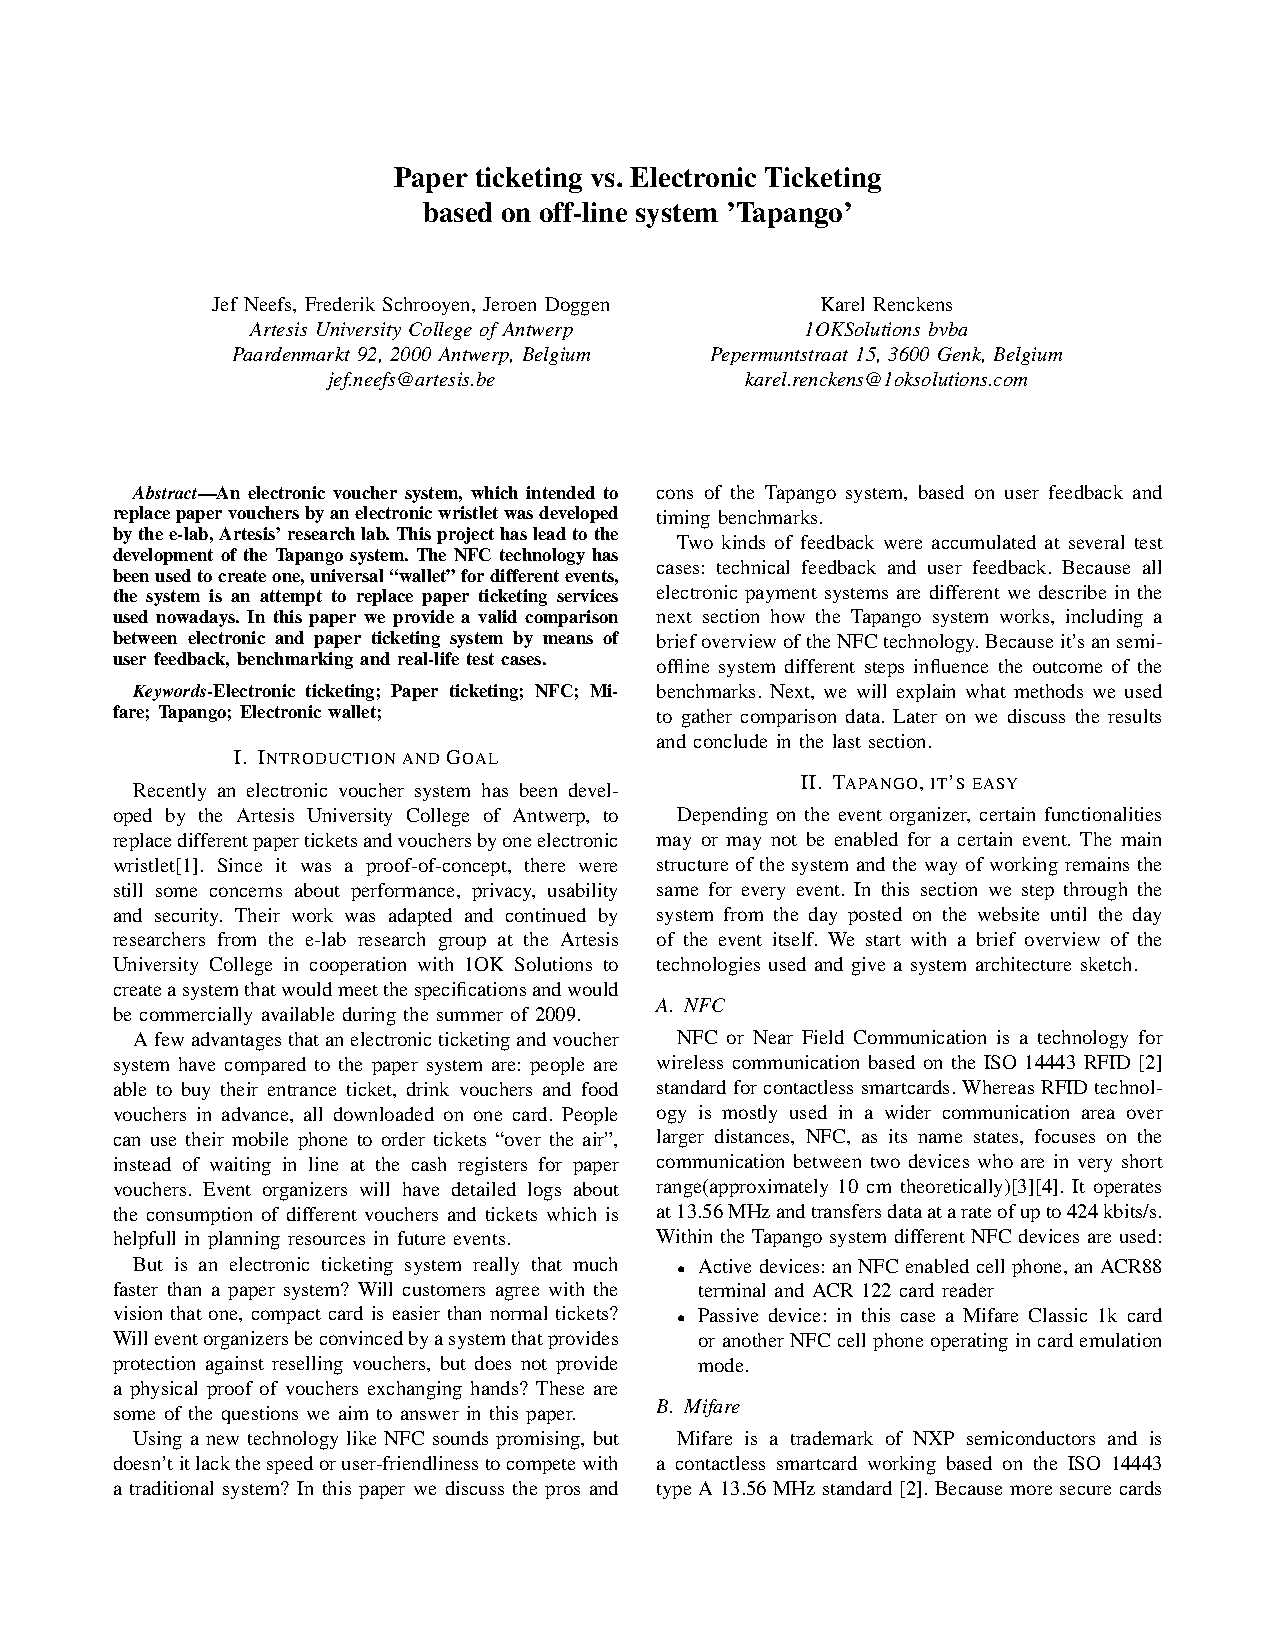
\includepdf[pages={1}]{includes/nfc2010.pdf}
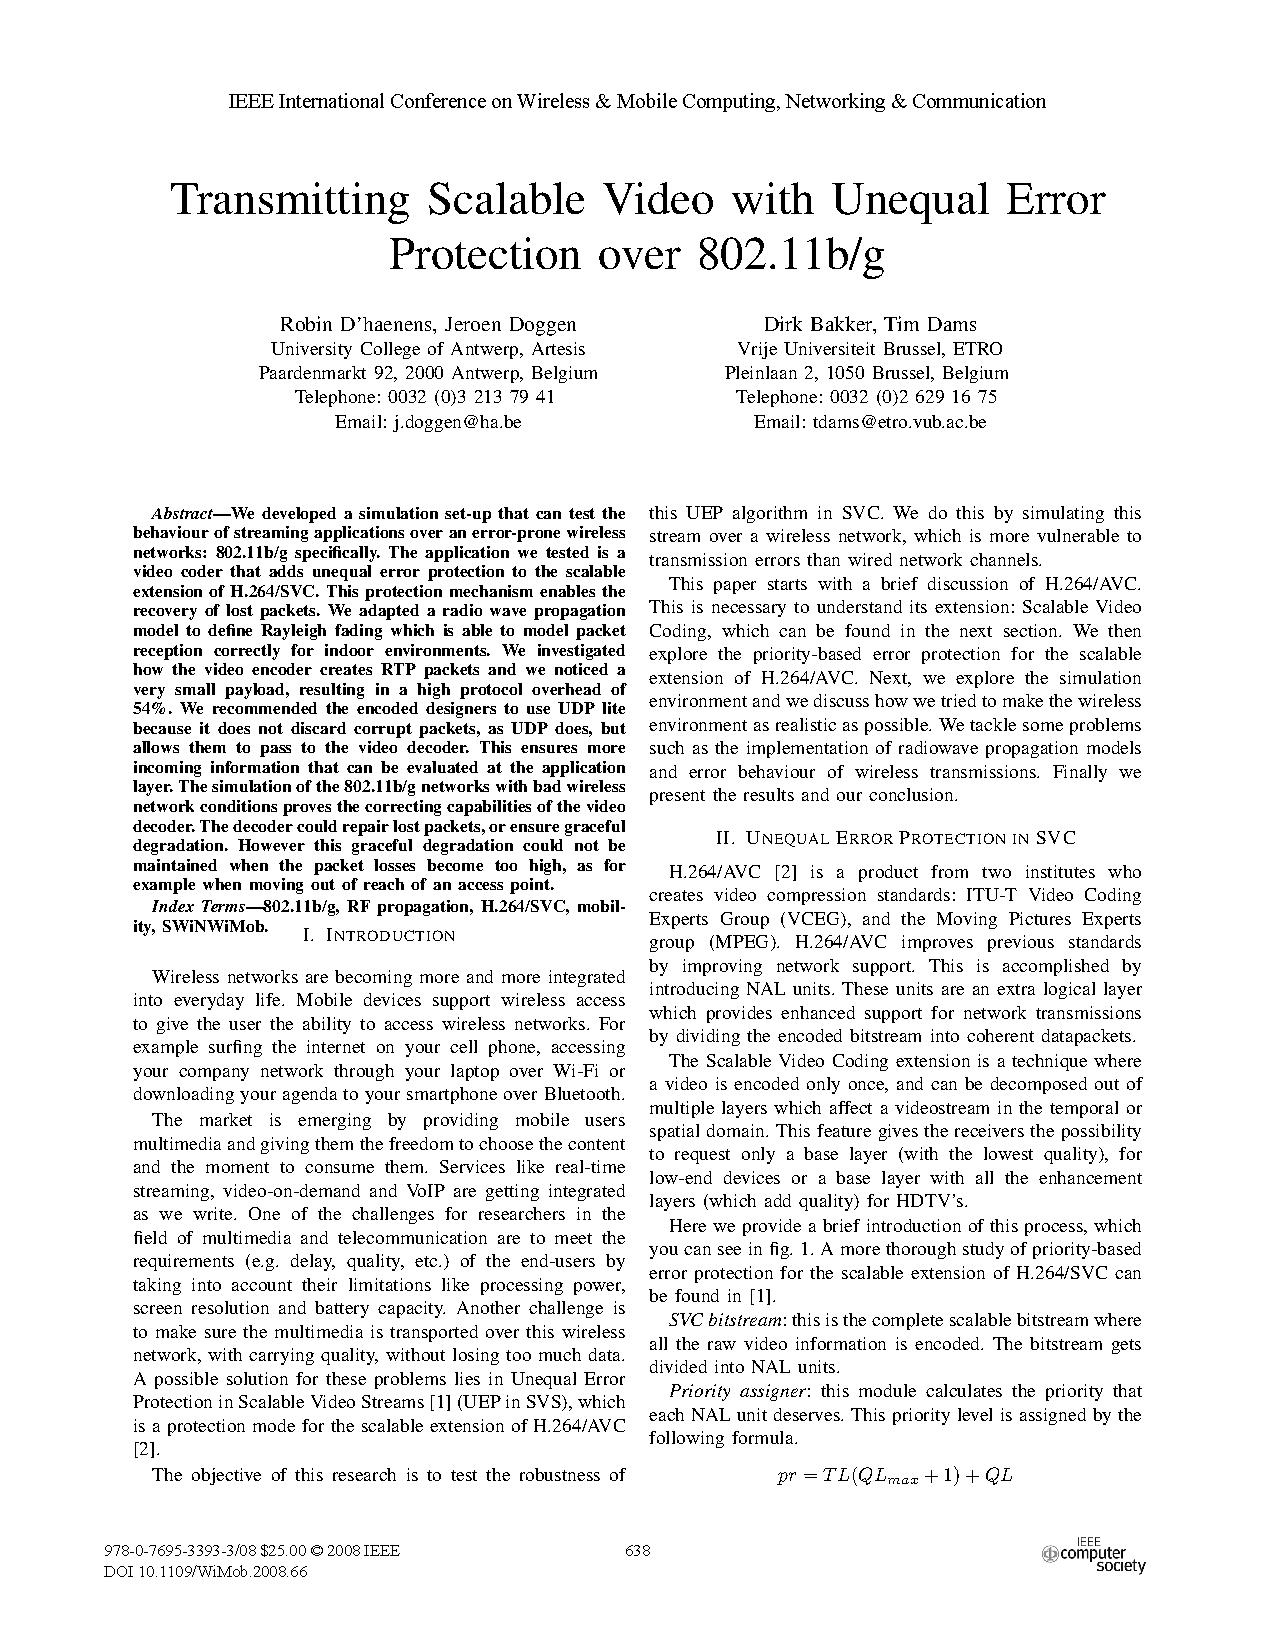
\includepdf[pages={1}]{includes/wimob2008.pdf}
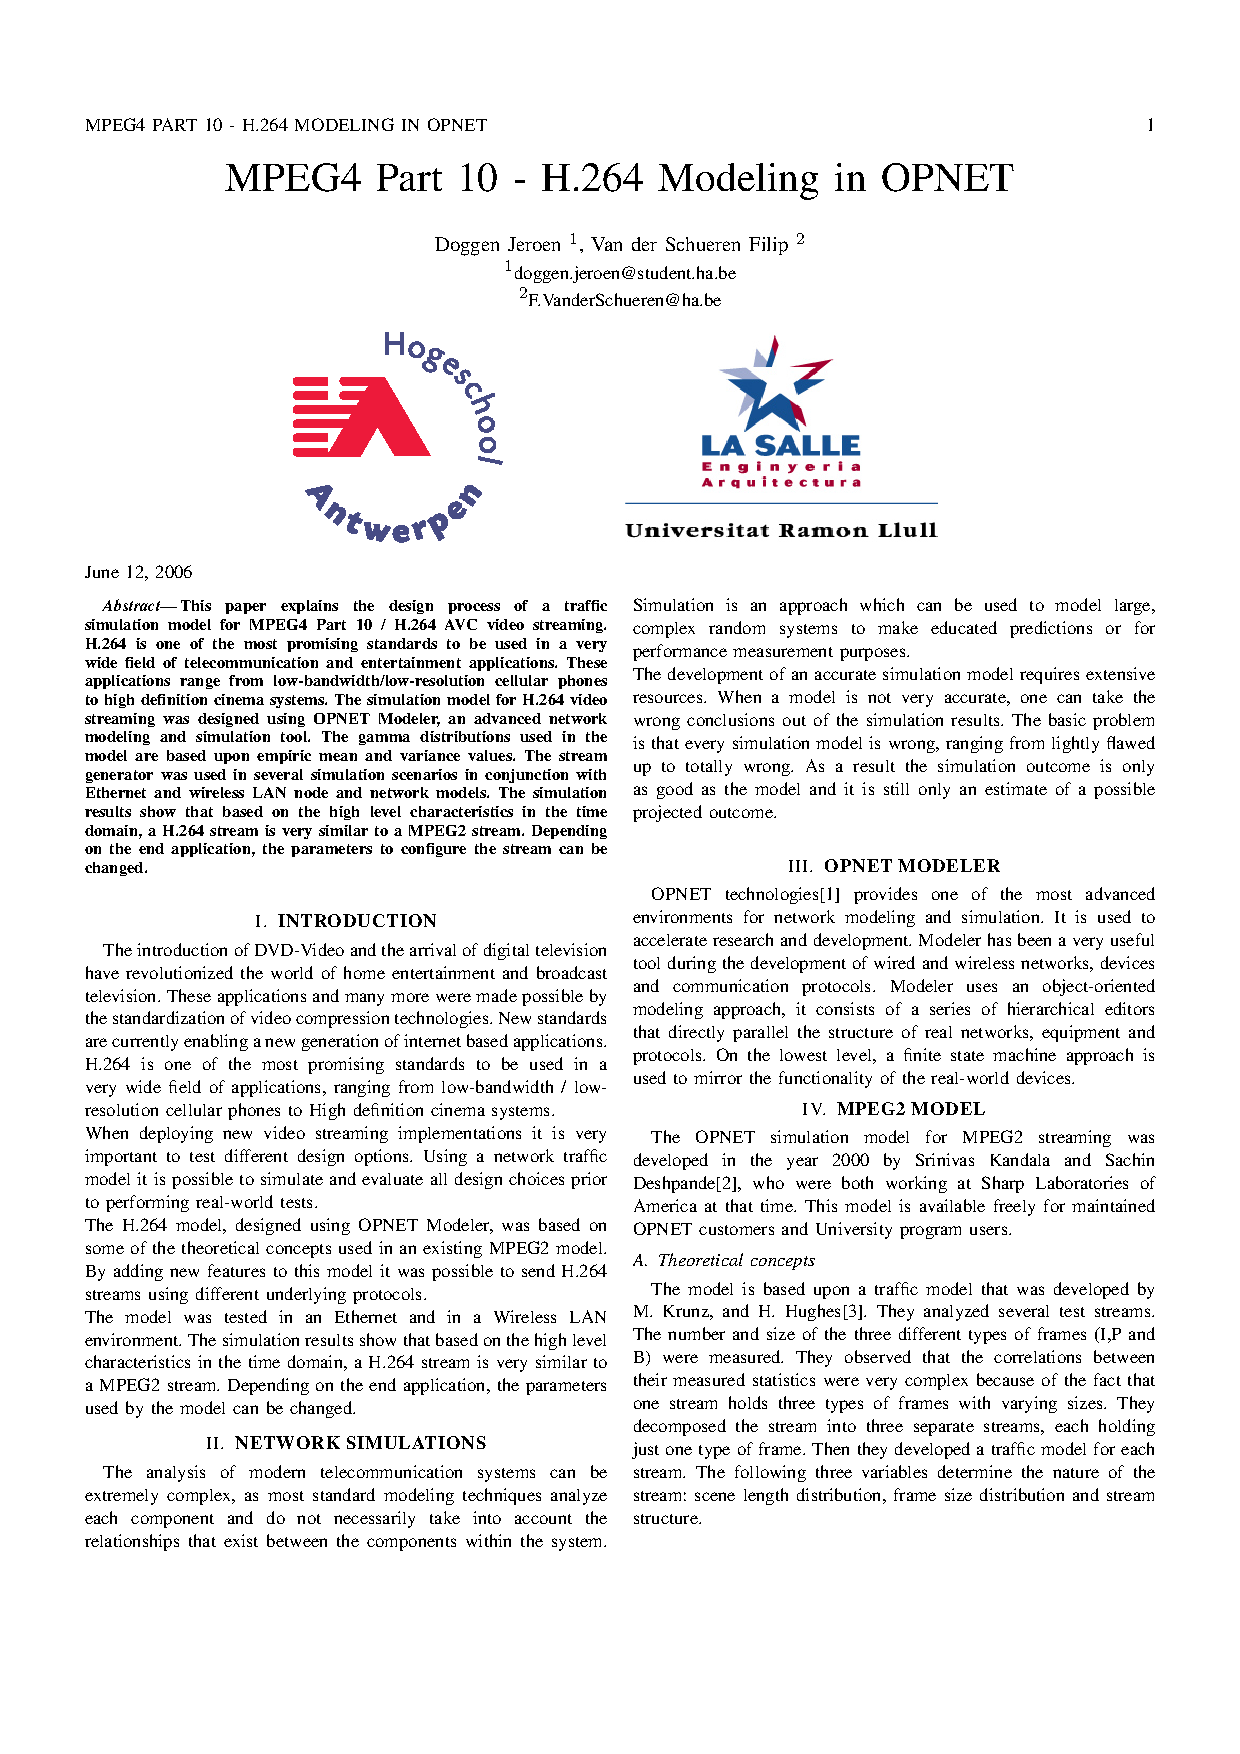
\includepdf[pages={1}]{includes/Doggen.pdf}
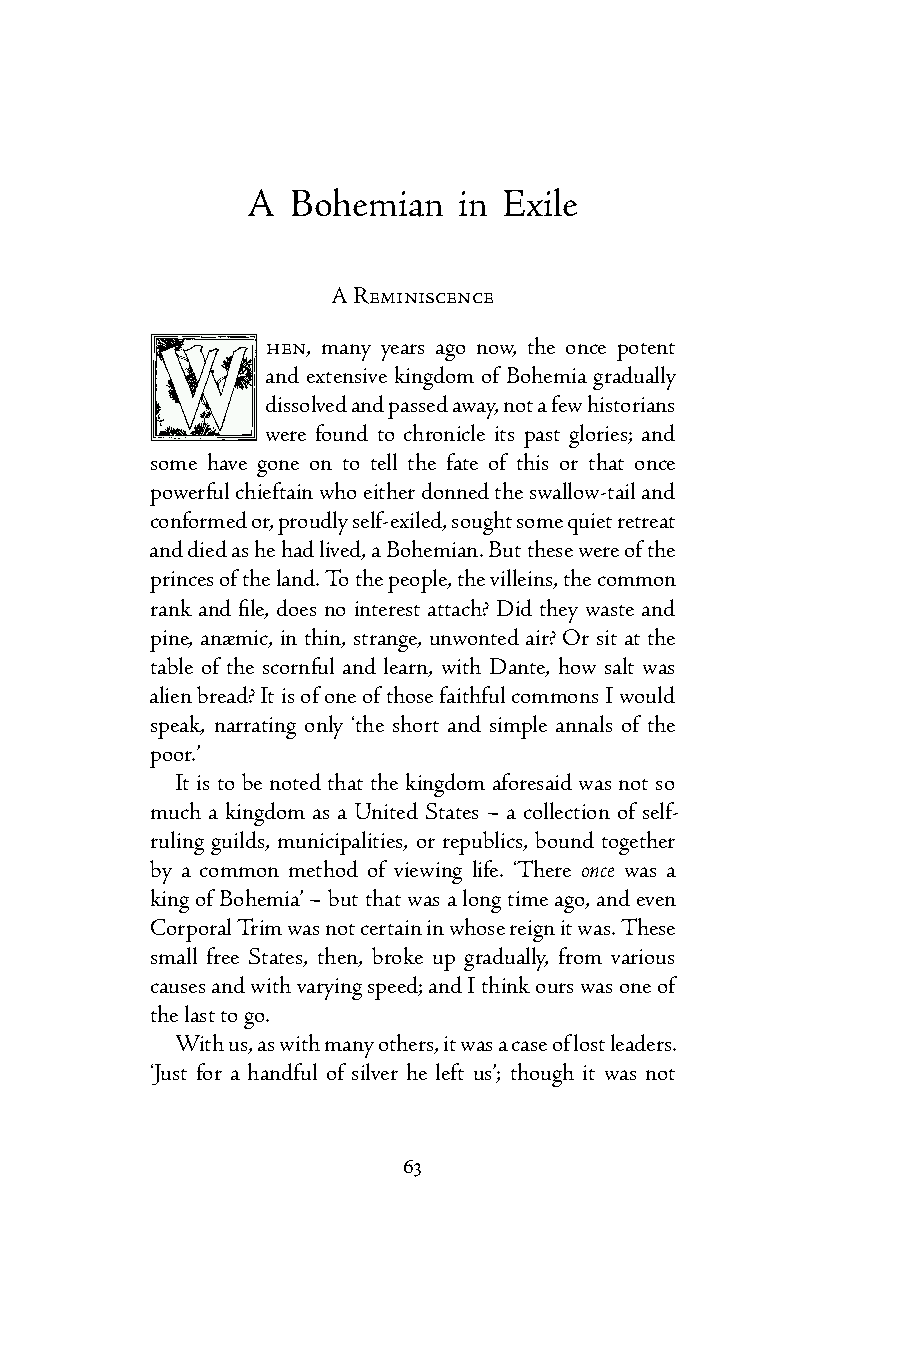
\includepdf[pages={1}]{includes/ex-book.pdf}
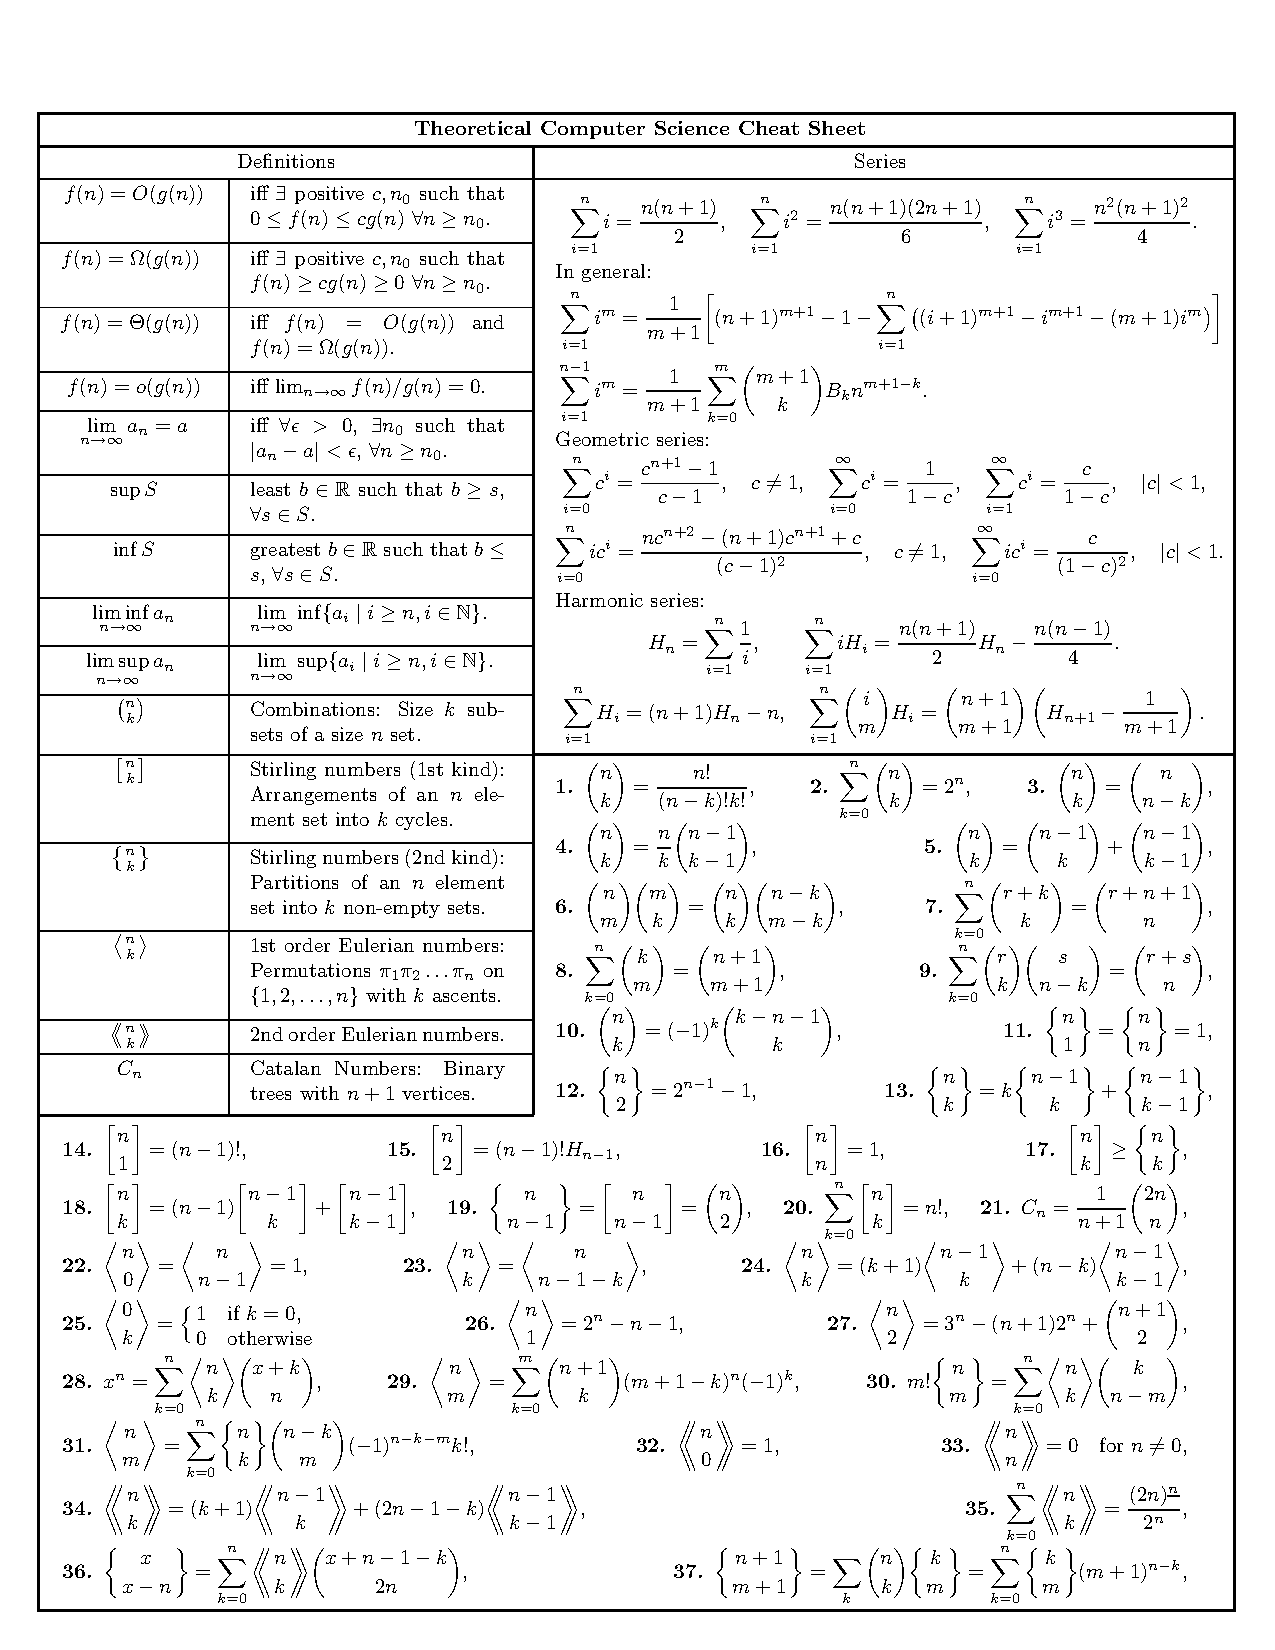
\includepdf[pages={1}]{includes/ex-cheat.pdf}
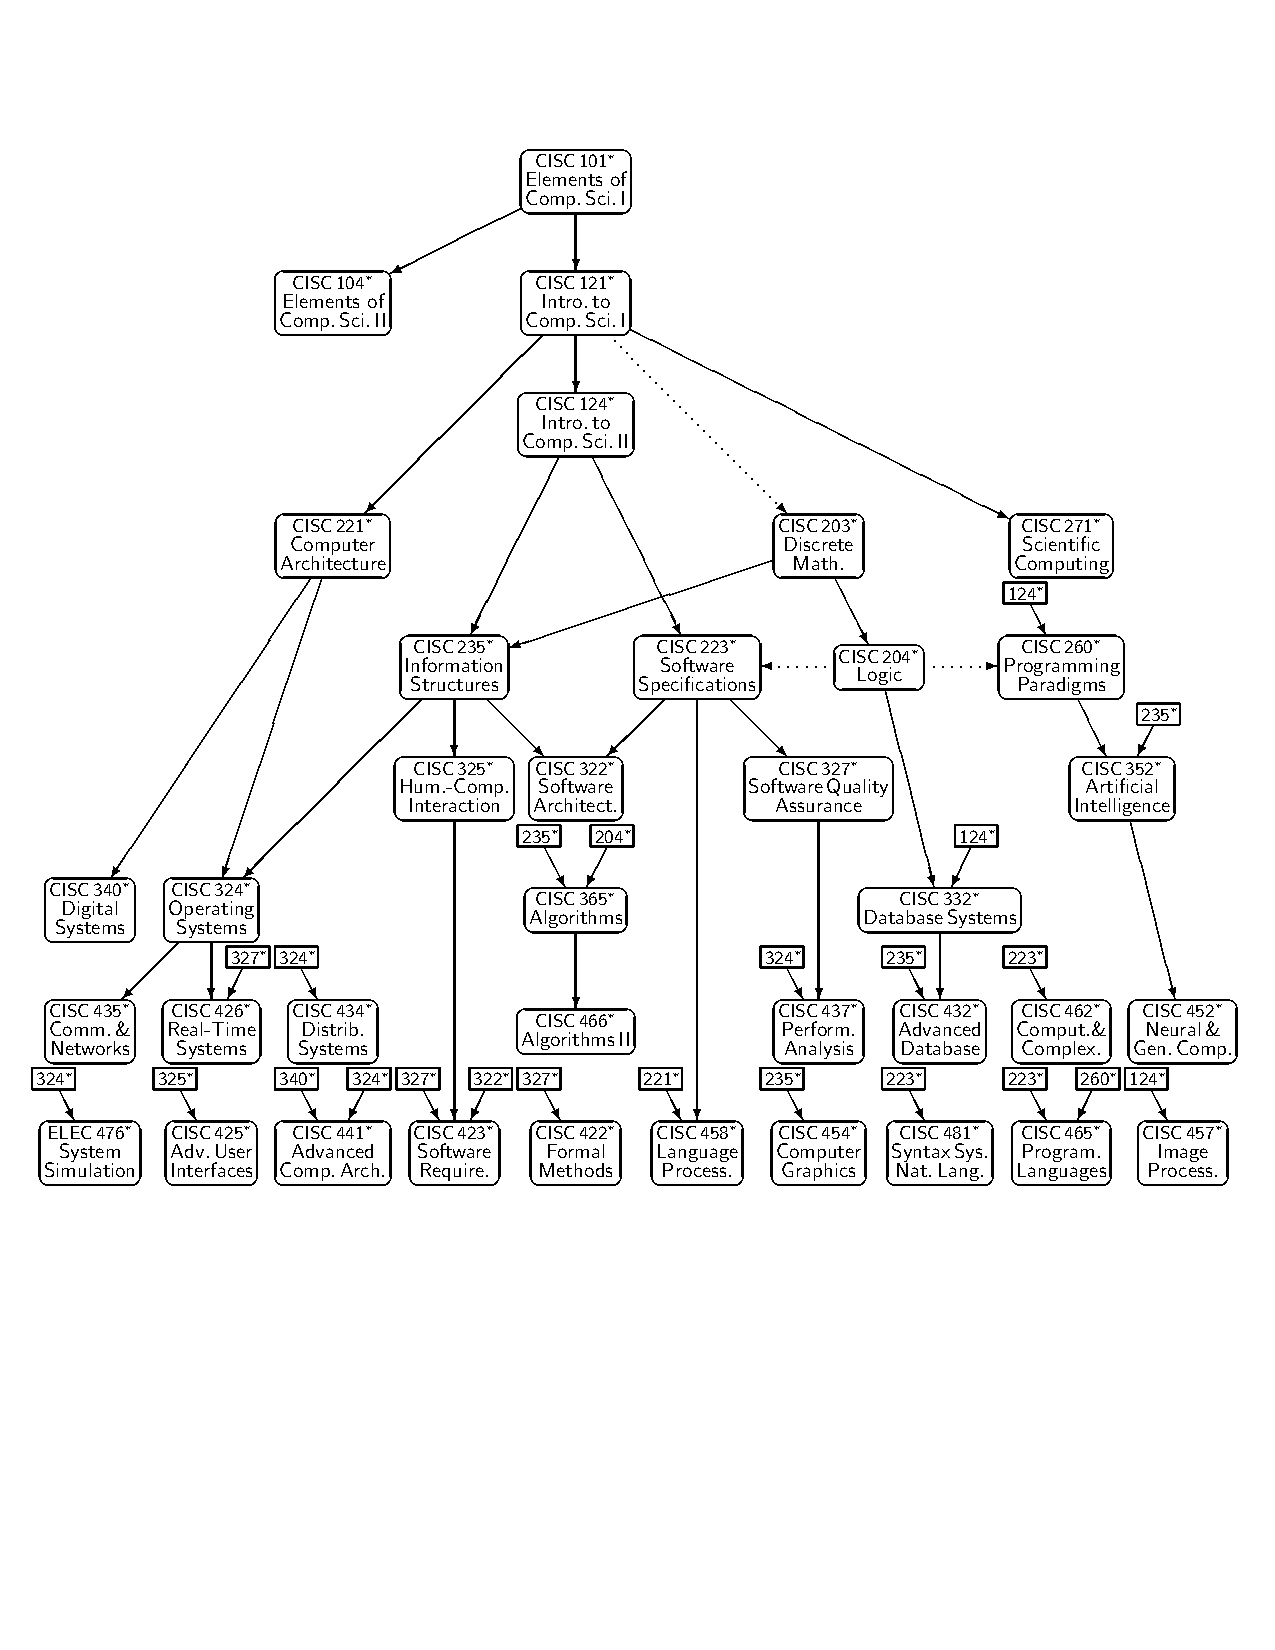
\includepdf[pages={1}]{includes/ex-diagram.pdf}
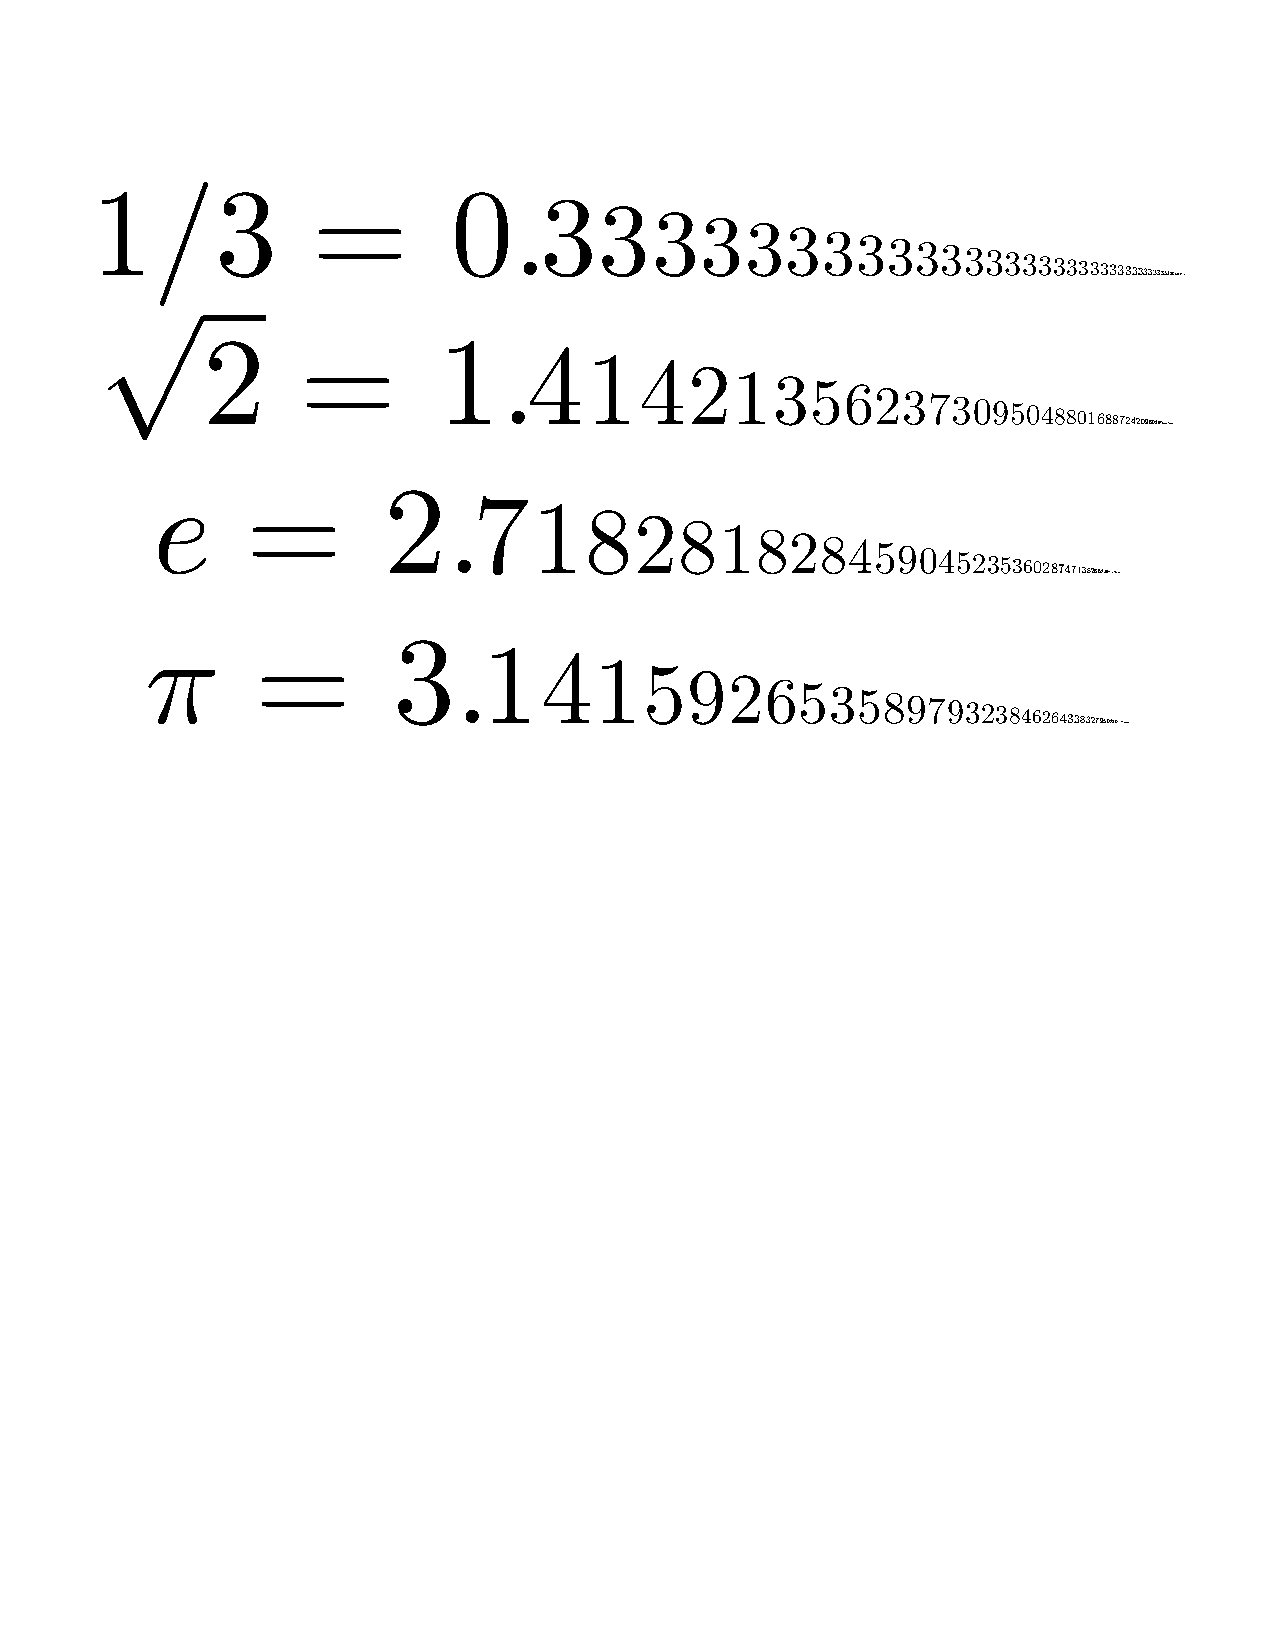
\includepdf[pages={1}]{includes/ex-dimin.pdf}
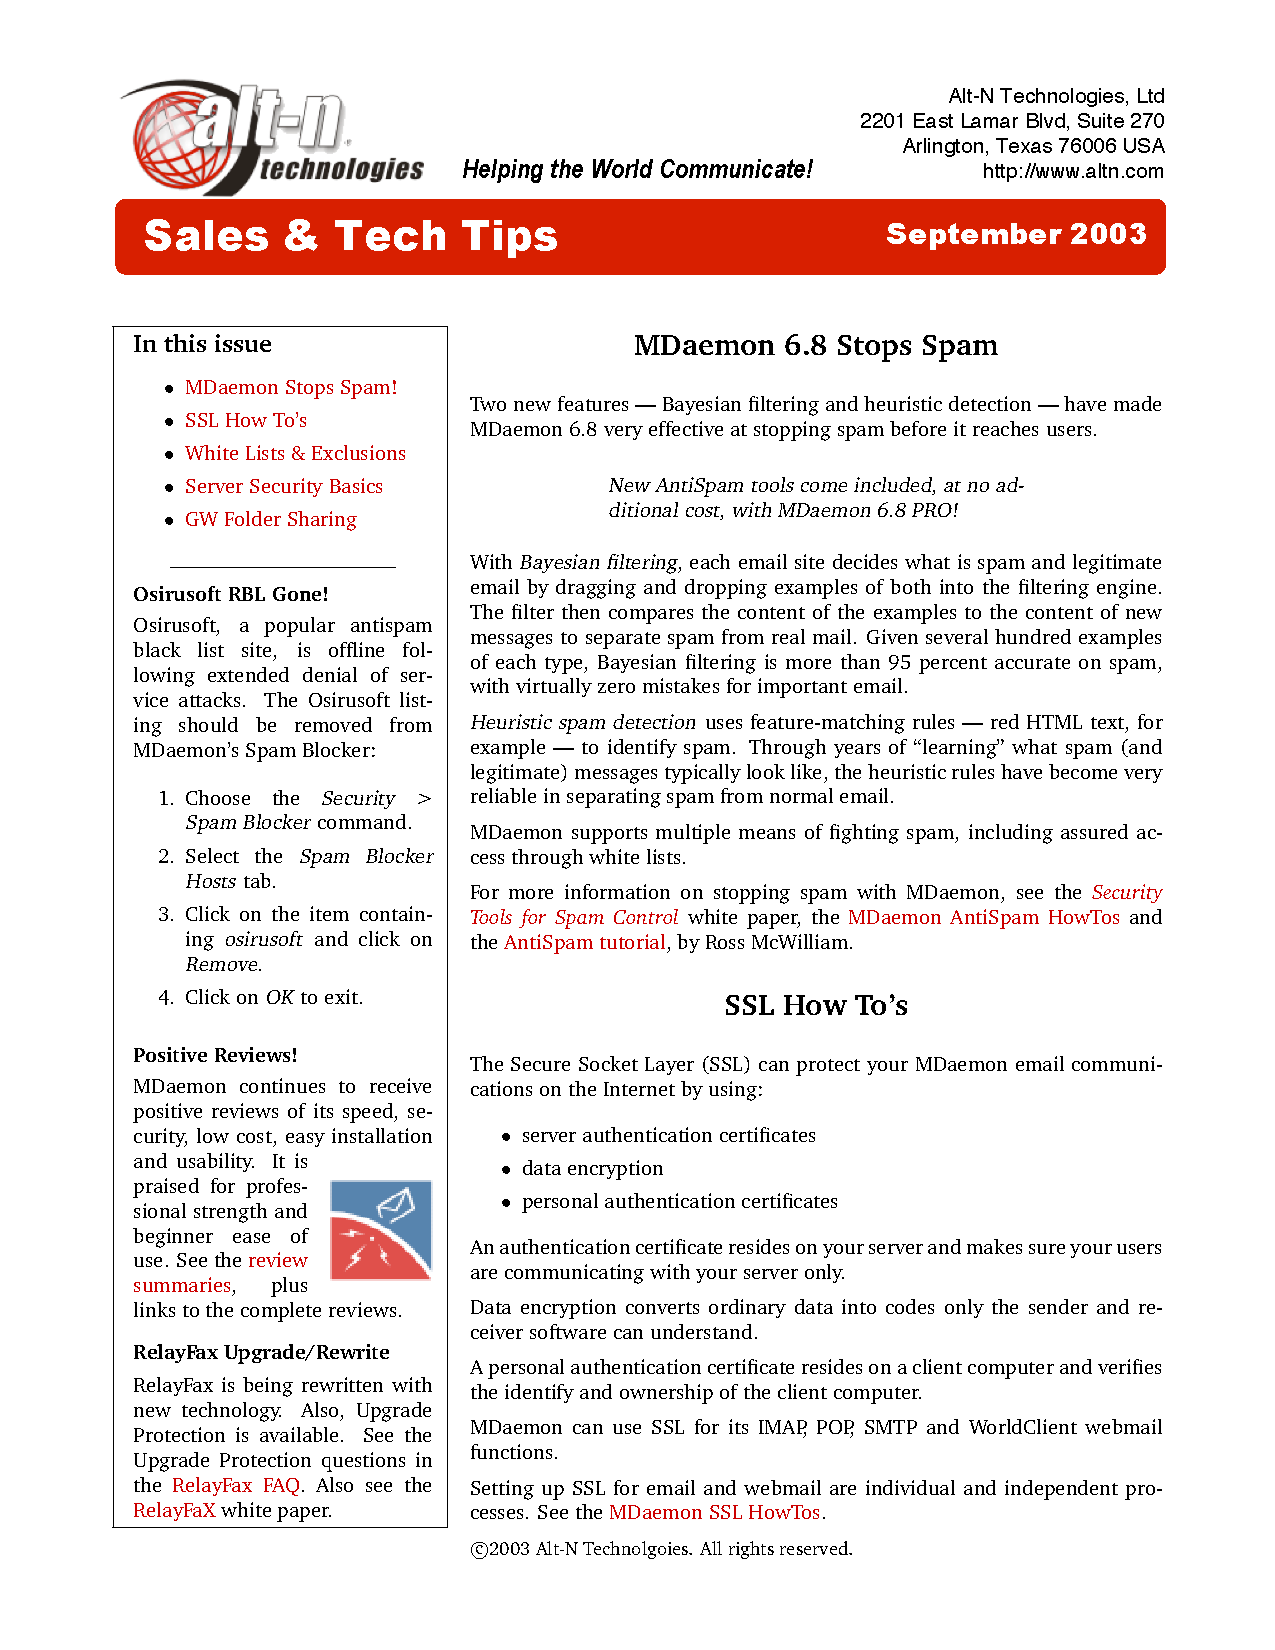
\includepdf[pages={1}]{includes/ex-letter.pdf}
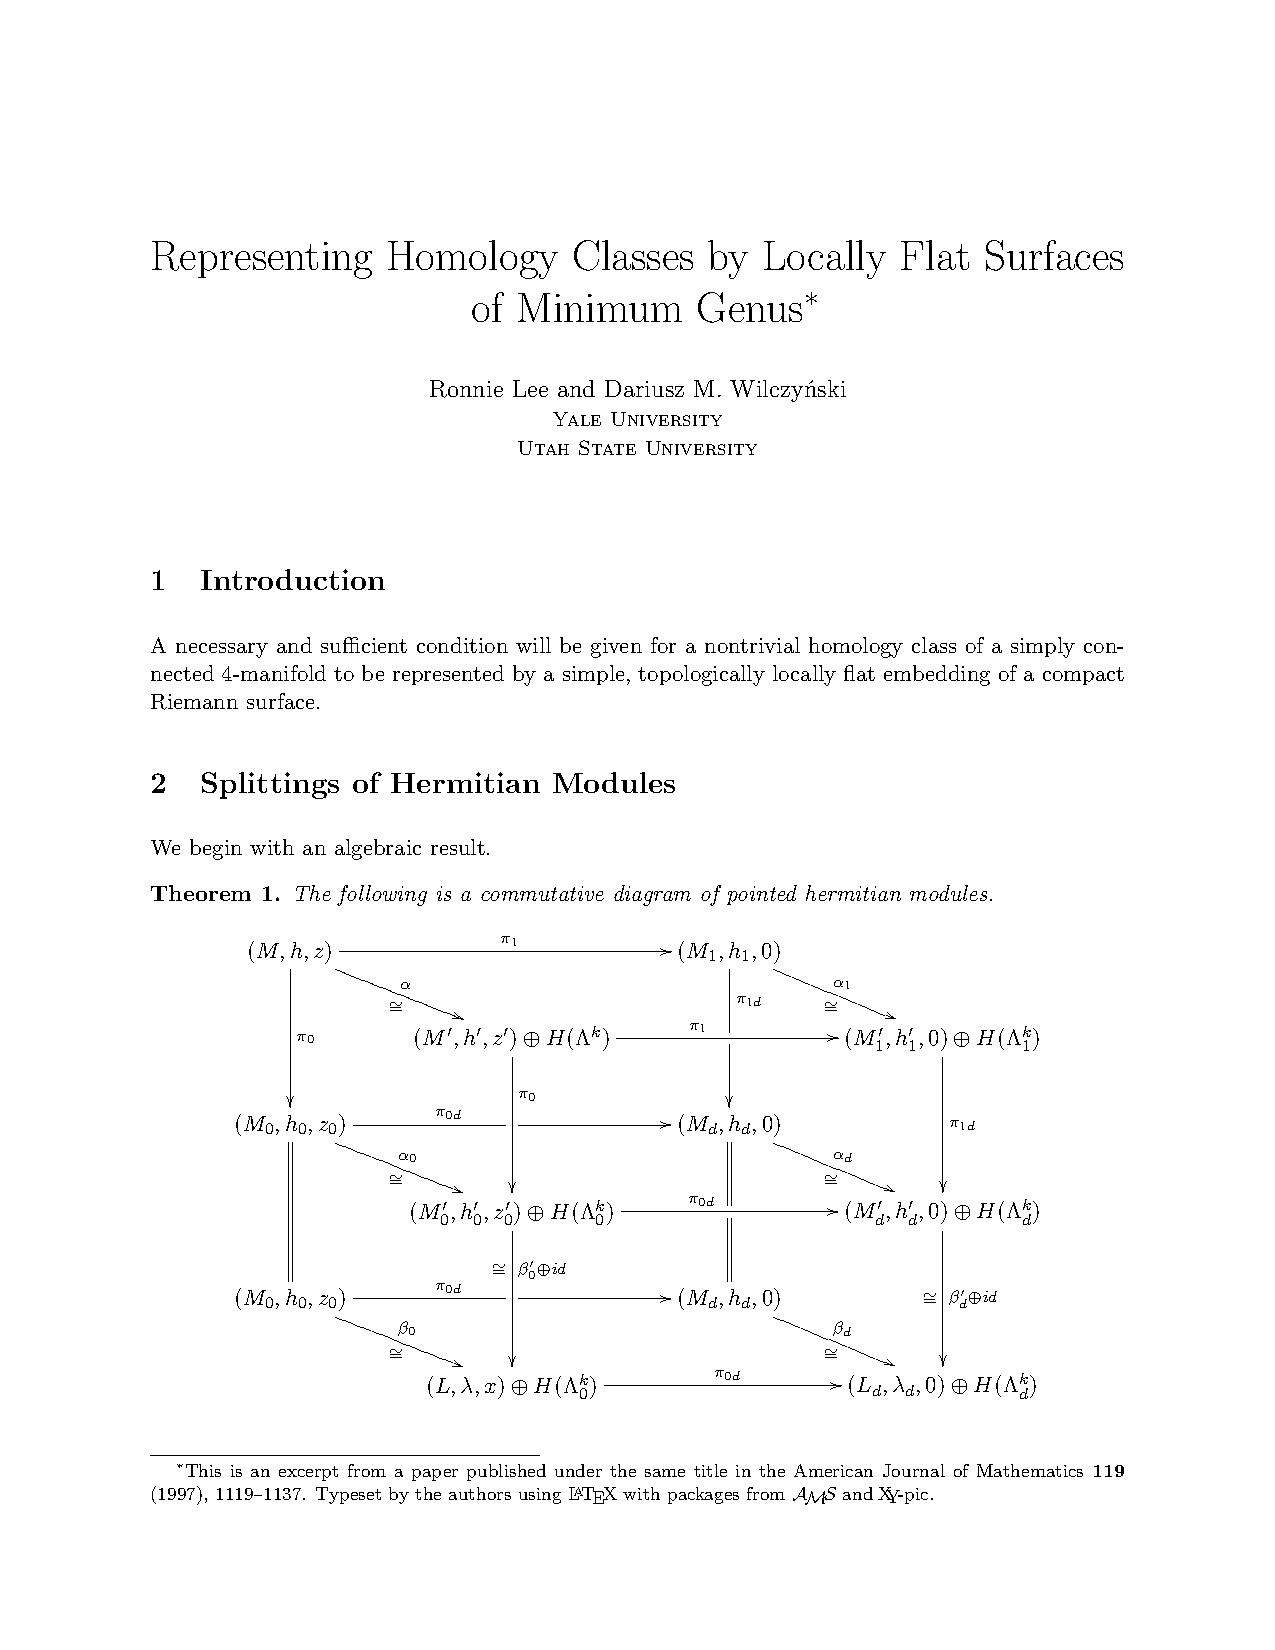
\includepdf[pages={1}]{includes/ex-math.pdf}
\includepdf[pages={2}]{includes/ex-phys.pdf}
\includepdf[pages={9}]{includes/ex-slide.pdf}
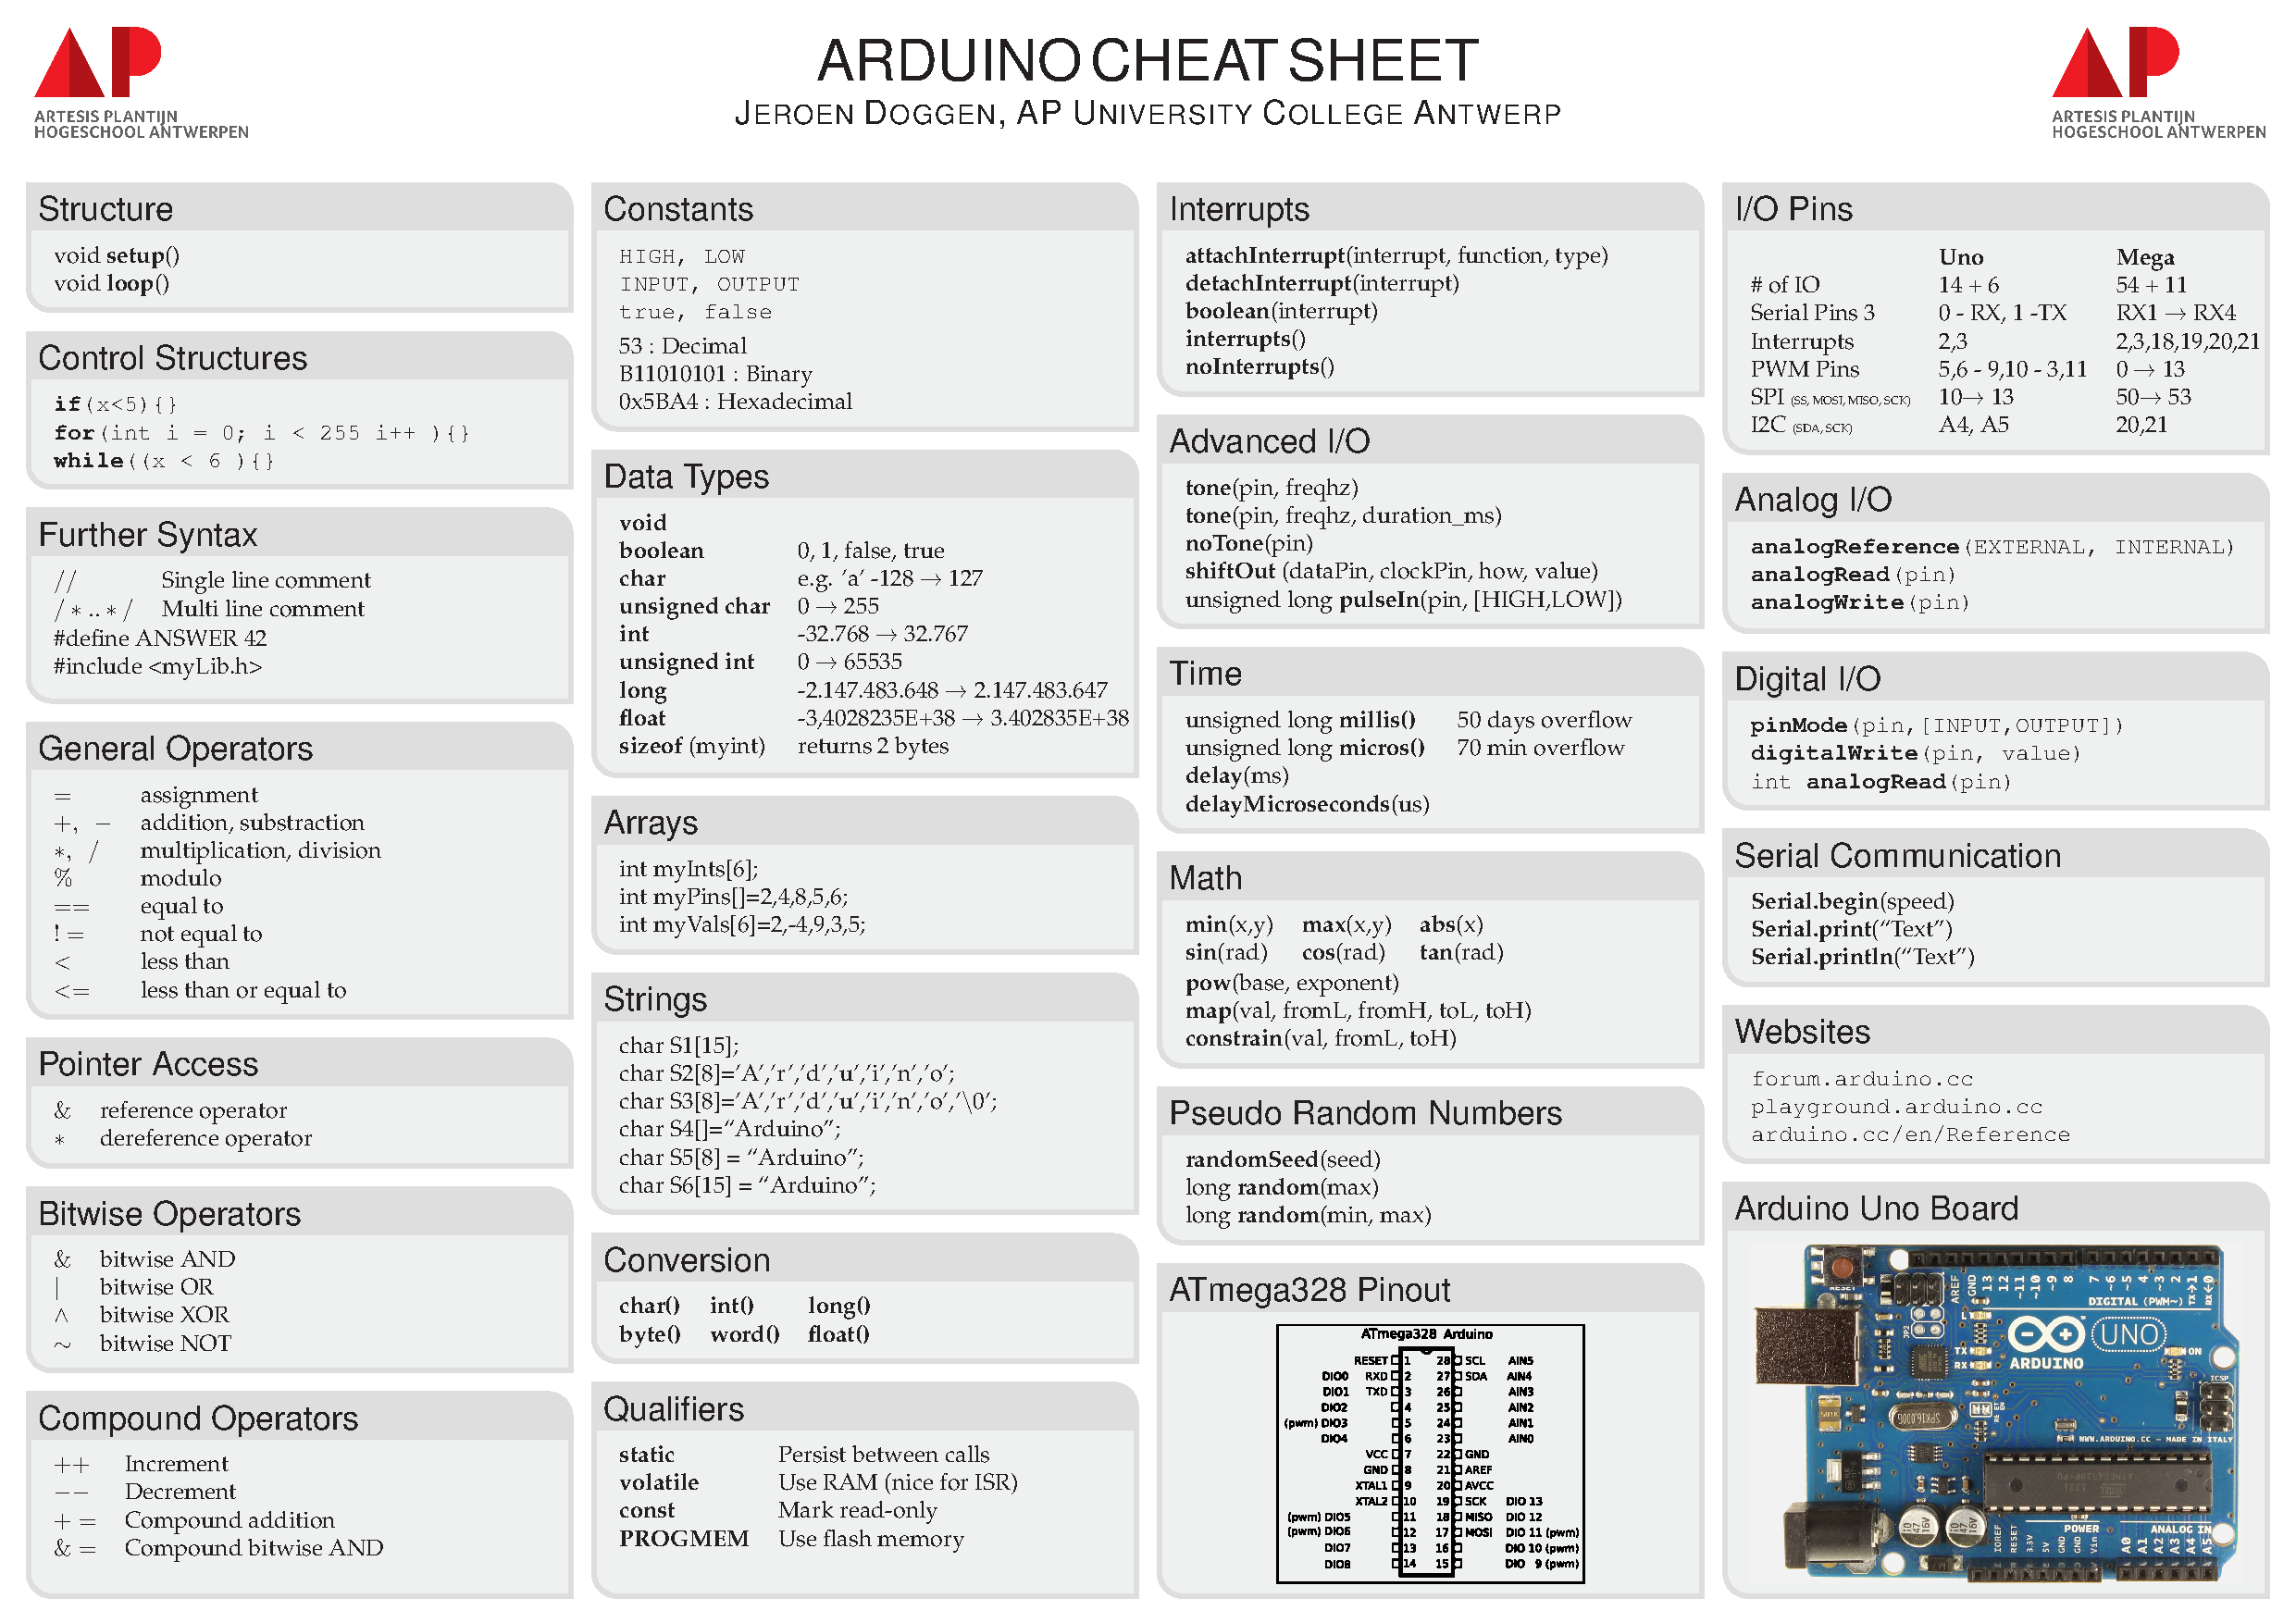
\includepdf[pages={1}]{includes/Arduino-Cheat-Sheet.pdf}

%%%%%%%%%%%%%%%%%%%%%%%%%%%%%%%%%%%%%%%%%%%%%%%%%%%%%%%%%%%%%%%%%%%%%%%%%%%%%%%%%%%%%%%%%%%%%%%%%%%%%%%%%%%%%%%%%%%%%%%%%%%%%%%%%%%%
\section{Meer \LaTeX $ $ informatie}
%%%%%%%%%%%%%%%%%%%%%%%%%%%%%%%%%%%%%%%%%%%%%%%%%%%%%%%%%%%%%%%%%%%%%%%%%%%%%%%%%%%%%%%%%%%%%%%%%%%%%%%%%%%%%%%%%%%%%%%%%%%%%%%%%%%%

\begin{frame}
\frametitle{Nuttige bronnen}
\begin{itemize}
 \item Not so short introduction to \LaTeX: \begin{tiny}
                                              \url{http://www.ctan.org/tex-archive/info/lshort/english/}
                                            \end{tiny}

 \item Universiteit Gent: \begin{tiny}
                           \url{http://latex.ugent.be/cursus.php}
                          \end{tiny}

 \item Monash University: \begin{tiny}
                           \url{http://www.csse.monash.edu.au/software/latex/}
                          \end{tiny}

 \item Niet onderschatten: \begin{tiny}
                            \url{www.google.com}
                           \end{tiny}
 \item \LaTeX $ $ cursus van het ``Association for Computing Machinery Antwerp Student Chapter (ACM):''
 \begin{tiny}
 \url{http://acmantwerp.acm.org}
 \end{tiny}
\end{itemize}
\end{frame}


% %%%%%%%%%%%%%%%%%%%%%%%%%%%%%%%%%%%%%%%%%%%%%%%%%%%%%%%%%%%%%%%%%%%%%%%%%%%%%%%%%%%%%%%%%%%%%%%%%%%%%%%%%%%%%%%%%%%%%%%%%%%%%%%%%%%%
% \subsection{Een korte geschiedenis}
% %%%%%%%%%%%%%%%%%%%%%%%%%%%%%%%%%%%%%%%%%%%%%%%%%%%%%%%%%%%%%%%%%%%%%%%%%%%%%%%%%%%%%%%%%%%%%%%%%%%%%%%%%%%%%%%%%%%%%%%%%%%%%%%%%%%%
% \includepdf[pages={-}]{1textalk.pdf}
% 
% %%%%%%%%%%%%%%%%%%%%%%%%%%%%%%%%%%%%%%%%%%%%%%%%%%%%%%%%%%%%%%%%%%%%%%%%%%%%%%%%%%%%%%%%%%%%%%%%%%%%%%%%%%%%%%%%%%%%%%%%%%%%%%%%%%%%
% \subsection{Slides \LaTeX cursus ACM Antwerp Student Chapter}
% %%%%%%%%%%%%%%%%%%%%%%%%%%%%%%%%%%%%%%%%%%%%%%%%%%%%%%%%%%%%%%%%%%%%%%%%%%%%%%%%%%%%%%%%%%%%%%%%%%%%%%%%%%%%%%%%%%%%%%%%%%%%%%%%%%%%
% \includepdf[pages={-}]{2slides2.pdf}



\end{document}